\chapter{Simulations results} \label{chap:results_sim}

\section{Introduction} \label{sec:intro_results_sim}

% Introduction to the chapter

\section{General response characterization of the baseline configuration} \label{sec:generalResponseCharact_results_sim}
  % 
  % -> Describe buckling without or before collapsing
  % -> Describe the evolution of the buckling for the normal case, 2 inner ribs and damping included
  %       - At the beginning, buckling appears at the same place than in the other cases, just after the inner big with higher x coordinate
  %       - Then, quickly buckling starts to appear in a more severe way close to the root. This is the point at which the local inestabilities are such that there is need of adding artificial damping factor in order to capture this dynamics. In \ref{fig:../figures/result-sim/energy} it is possible also to see the abrupt change in the external work put into the system. After this point, the artifial damping allows the simulation to continue, however, the static dissipation through automatic estabilization is neglectable in comparison with the external work.

  In this section, the general response of the model will be characterized. For the wing-box, the nominal value of its characteristic parameters are those shown in Table \ref{tab:parameters_wing-box}, while Tables \ref{tab:parameters_lattice} and \ref{tab:parameters_wing-box} contain the nominal values of the main parameters for the chiral lattice and the ribs, respectively. Also, the baseline configuration will incorporate a pair of inner ribs and the load will be applied on a single mesh node on the upper flange of the tip rib, as described in Subsection \ref{subsec:load_results_model}.

  In th simulation, automatic stabilization will be performed through the inclusion of artificial constant damping factor. For this case, the response of the structure when 65\% of the prescribed load has been applied is the one shown in Figure \ref{fig:1-UR}. It can be seen that buckling starts and it is more severe in the ligament located just after the inner rib located closer to the root. In a further load increment, buckling phenomena moves backwards and those ligaments located close to the root and with a higher $y$ coordinate, start to deform even more severely. At this point, the structure collapses and the twist increases for smaller increments in the applied load. This can be seen in Figure \ref{fig:2-UR}.

  \begin{figure}[!htpb] %First step in the deformation 
    \centering
    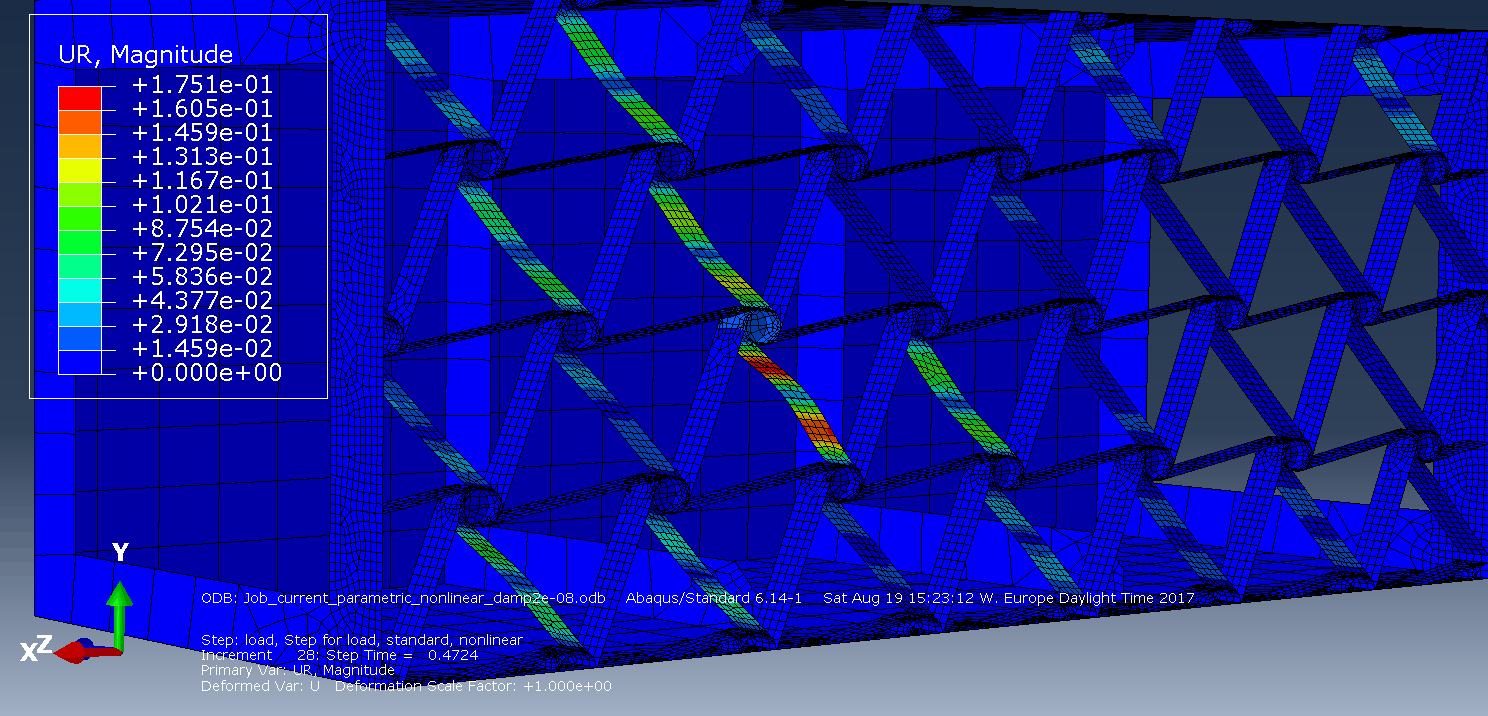
\includegraphics[width=0.8 \textwidth]{../figures/result-sim/1-UR}
    \caption[Baseline model response when the fraction of load applied equals to 63\% of the prescribed load (700 N)]{Baseline model response when the fraction of load applied equals to 63\% of the prescribed load (700 N). Buckling has appeared and it is more severe on the chiral ligament located closer to the inner rib located closer to the root.}\label{fig:1-UR}
  \end{figure}

  \begin{figure}[!htpb] %First step in the deformation 
    \centering
    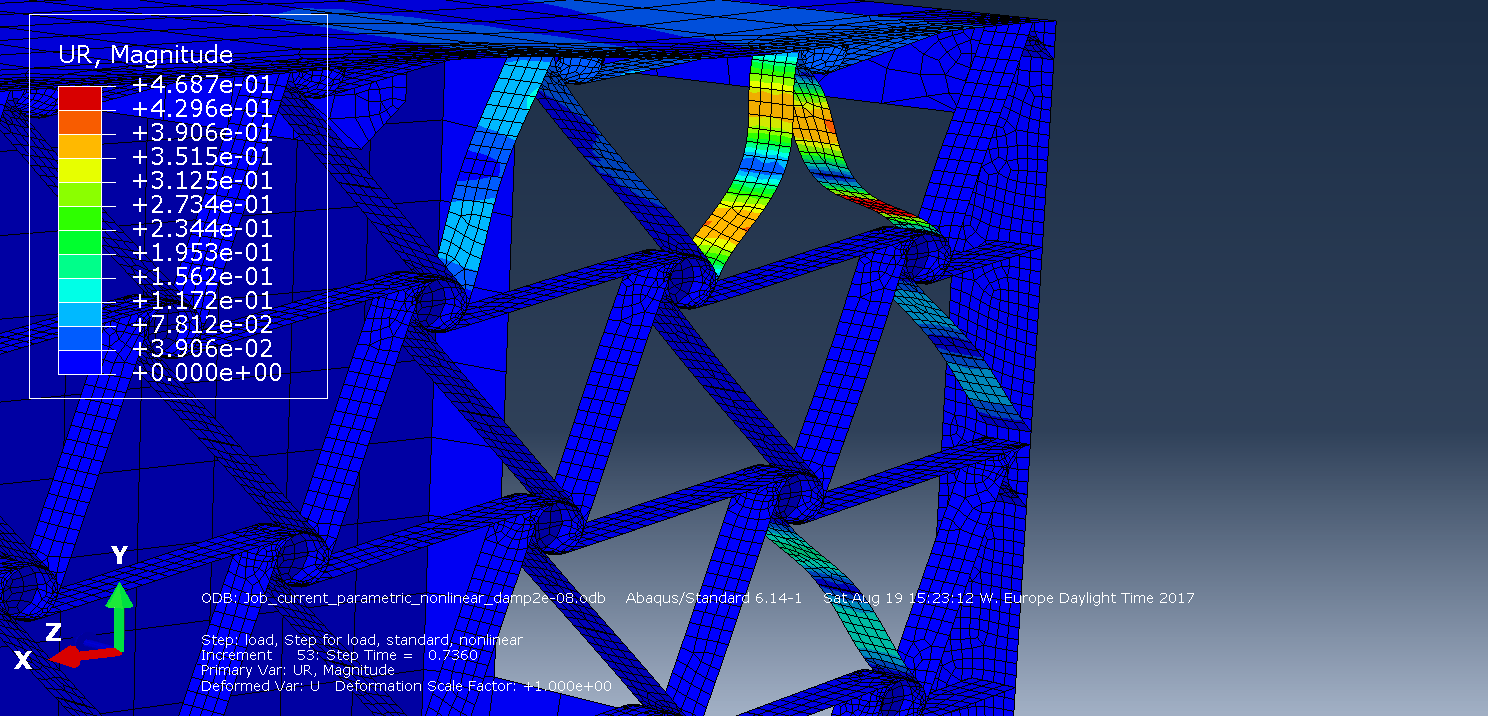
\includegraphics[width=0.8 \textwidth]{../figures/result-sim/2-UR}
    \caption[Baseline model response when the fraction of load applied equals to 80\% of the prescribed load (700 N)]{Baseline model response when the fraction of load applied equals to 80\% of the prescribed load (700 N). Severe buckling appears in those chiral ligaments located at the root and with a higher $y$ coordinate. This is the point when the structure collapses and the twist increases for smaller increments in the applied load.}\label{fig:2-UR}
  \end{figure}

  This is the point at which the local instabilities are such that there is need of adding artificial damping factor in order to capture this dynamics. After this point, the artificial damping allows the simulation to continue. Special care needs to be taken in order not ensure that the inclusion of artificial damping factor is not leading to inaccurate results due to over-damping of the structure. This can be done why comparing the fraction of the static energy that it is dissipated compared to the external work that its put into the system. The Figure \ref{fig:energy} makes this comparison possible. It can be seen that effectively, the static dissipation through automatic stabilization is negligible in comparison with the external work. This figure also shows the abrupt increment in external work at the point where the structure collapses due to sudden buckling of the chiral ligaments.

  \begin{figure}[!htpb] %Energy plot
    \centering
    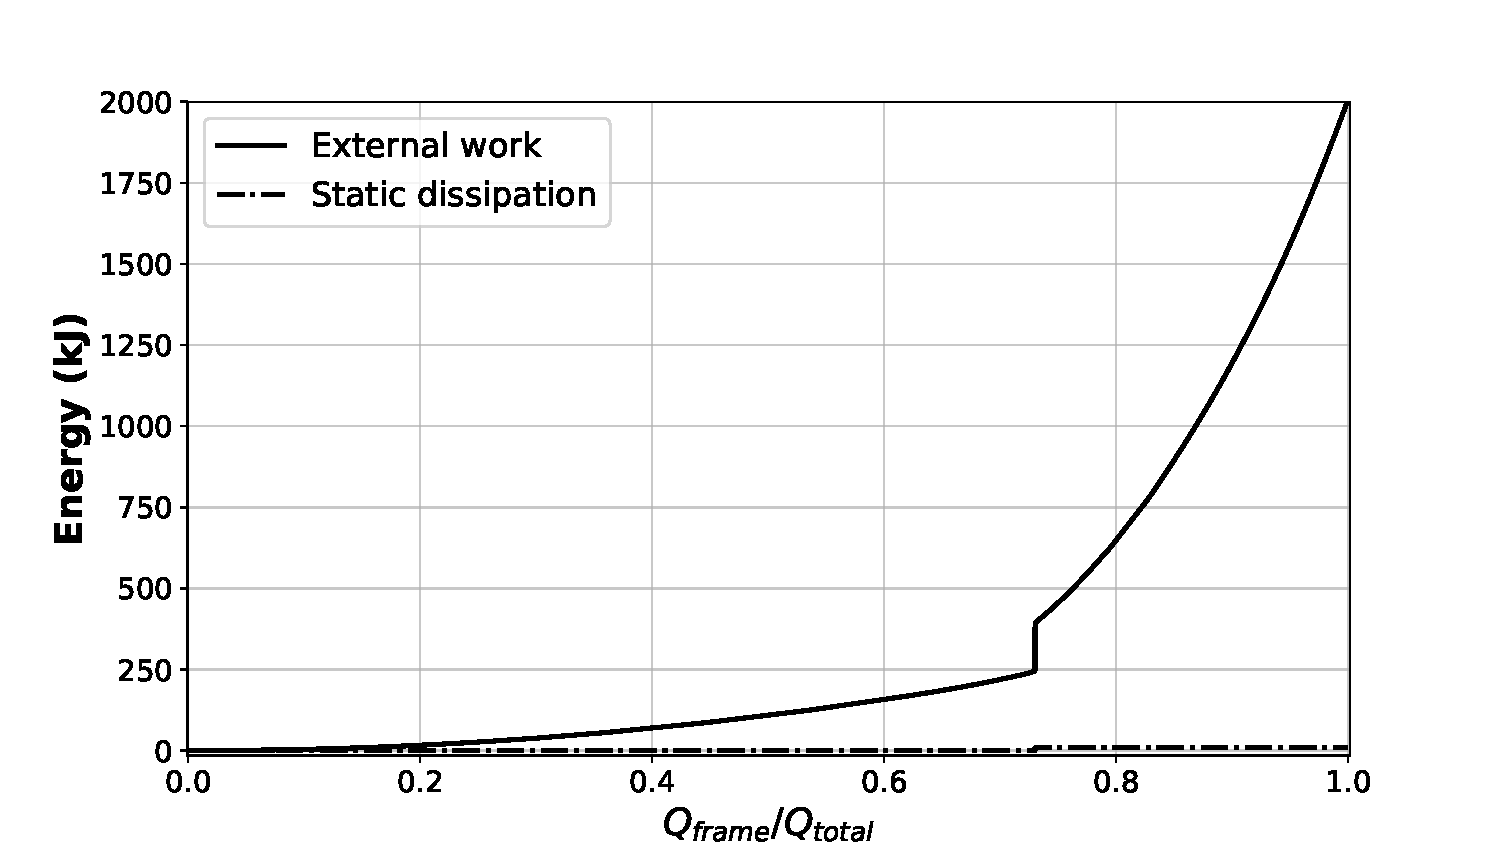
\includegraphics[width=0.8 \textwidth]{../figures/result-sim/energy}
    \caption[External work and static dissipation for a simulation of the baseline configuration]{External work and static dissipation for a simulation of the baseline configuration. It can be seen that the static dissipation through automatic stabilization is negligible in comparison with the external work showing that the inclusion of artificial damping factor is unluckily to be leading to inaccurate results. The abrupt change in the external work shows the point where structure collapses due to sudden buckling of the chiral ligaments.}\label{fig:energy}
  \end{figure}

  In order to see the overall system response as load increases, a load-displacement curve can be plotted. The Figure \ref{fig:forceDisplacement-far} shows the typical twist variation as the load is increased. On this plot, the results from the nonlinear simulations are shown as the set of scatter points while the dotted line represents the forecast final twist from the linear simulation. In the case shown, the linear simulation arises a twist at the tip $\phi_{\mathrm{tip}}$ equal to $-0.196$ degrees while the nonlinear simulation predicts a final twist of $-1.248$ degrees. This shows how the problem under study is highly nonlinear.

  The nonlinear response also shows the point where the structure collapses that its located at the point where approximately $80\%$ of the load has been applied. The deformation state of the structure at this point was the one shown in Figure \ref{fig:2-UR}. The plot also, shows another point where the deformation rapidly changes. This point is approximately located at the point where the load fraction is $82\%$. This shows the structure entering in the second stage of its deformation. Here, the buckling is more generalized and buckling appears in more ligaments apart from those at the root. This can be seen in Figure \ref{fig:3-UR}. The location of this second deformation breakdown varies widely with the choose of parameters.

  \begin{figure}[!htpb] %Energy plot
    \centering
    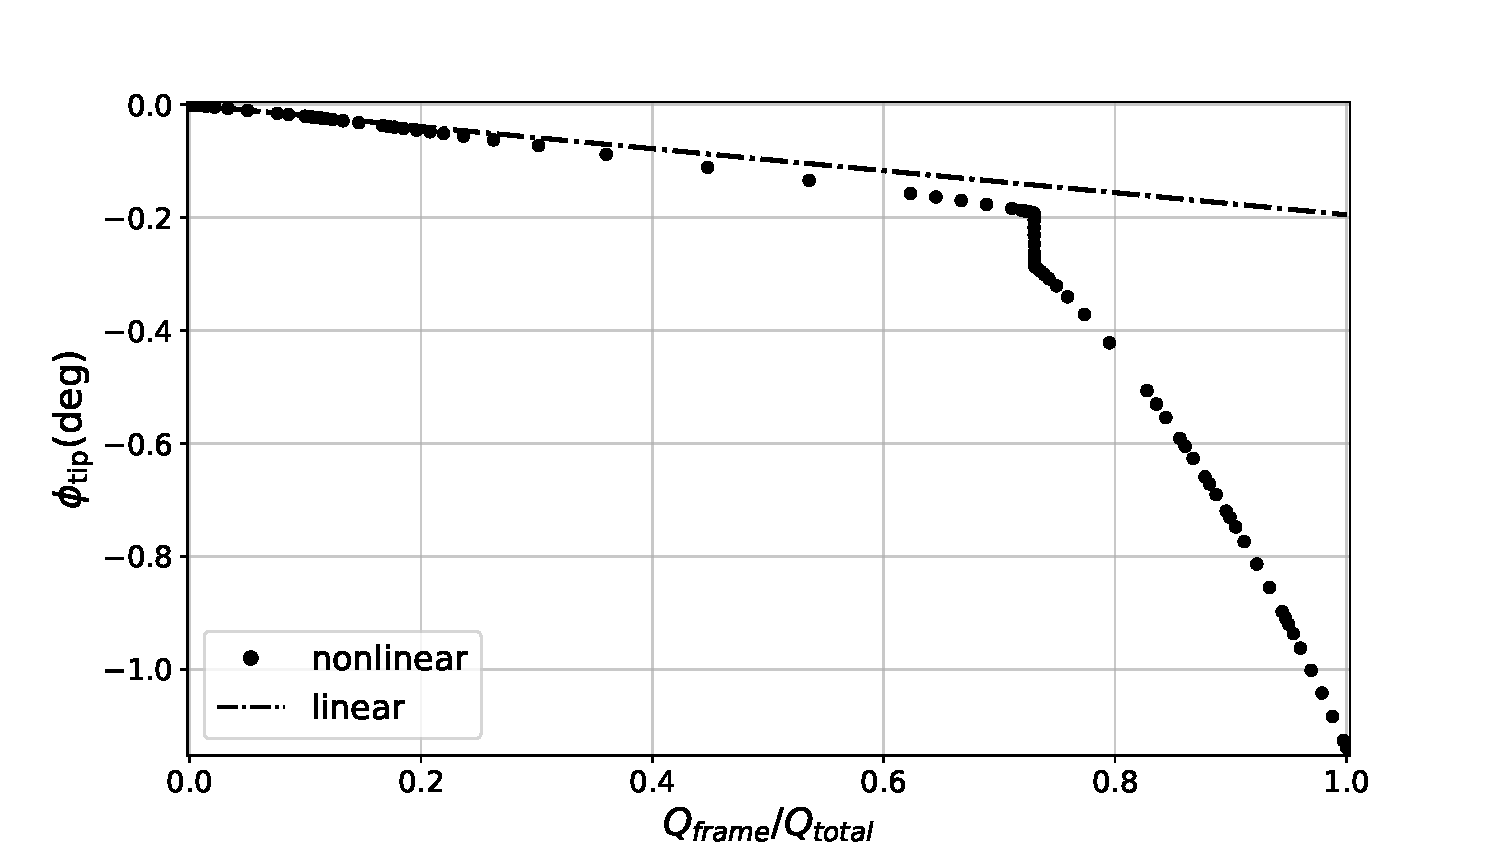
\includegraphics[width=0.8 \textwidth]{../figures/result-sim/forceDisplacement-far}
    \caption[Force-displacement curve for the baseline configuration]{Force-displacement curve for the baseline configuration. Two breakdowns for the buckling deformation are shown in the plot. The first one is located at the point where the fraction of applied load equals to $80\%$ and the second one at the point where the fraction is $82\%$.}\label{fig:forceDisplacement-far}
  \end{figure}

  \begin{figure}[!htpb] %Energy plot
    \centering
    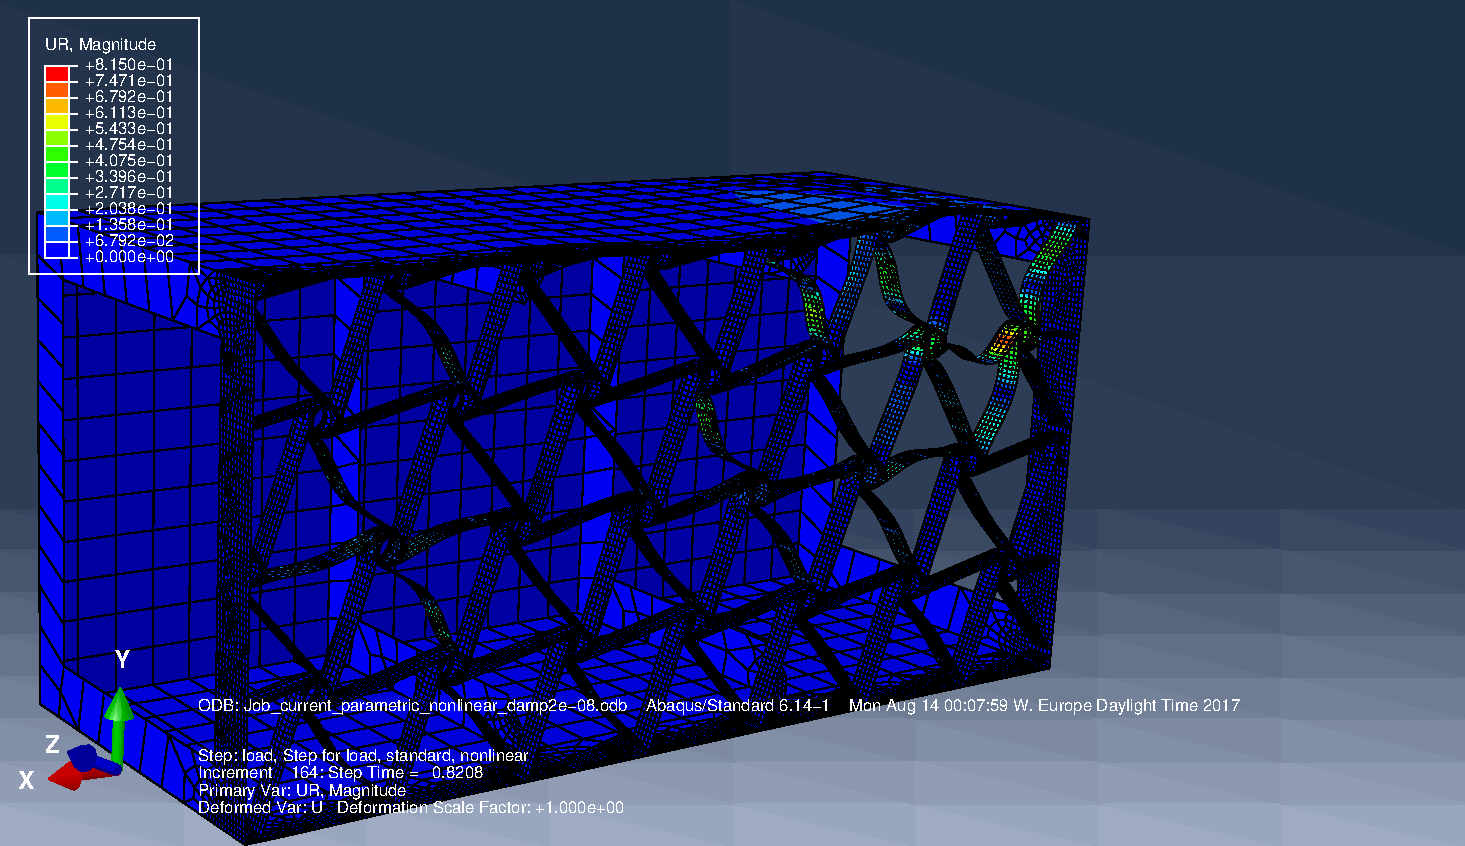
\includegraphics[width=0.8 \textwidth]{../figures/result-sim/3-UR}
    \caption[Baseline model response when the fraction of load applied equals to 82\% of the prescribed load (700 N)]{Baseline model response when the fraction of load applied equals to 82\% of the prescribed load (700 N). In this case, not only the ligaments located at the root show severe buckling but also, other located at different points of the chiral lattice has started to buckle at the same time, inducing rapidly growing deformation for small increments in load.}\label{fig:3-UR}
  \end{figure}
  
\clearpage
\section{Parametric study on the computational model} \label{sec:computationalParametricStudy_results_sim}
  %
  % *Cbox-t: Minimum seems to be 0.8. For less values, the simulation crashes.
  The aim of this section is to show the effect of each parameter on the nonlinear response of the structure. The parameters that will be included in the analysis are the following:

  \begin{itemize}
    \item Wing-box thickness \boxt
    \item Number of unit cells in the transversal direction $M$
    \item Number of unit cells in the spanwise direction $N$
    \item Chiral node depth \chiB
    \item Chiral node radius \chir
    \item Chiral lattice thickness \chit
    \item Chiral ligament half length \chiL
    \item Dimensionless ligament eccentricity \chie
  \end{itemize}

  \subsection{Wing-box thickness} \label{subsec:Cbox_t_para}
    %Summary of results
    %   - Range: 0.8, 1, 1.2, 1.4
    %   - This parameters has high influence in the appearance of buckling or not
    %   - Force displacement plot
    %       - For the one close. It is possible to see that for all the cases except one, the response is linear at the beggining, but non-linearities become relevant when the applied load is \%20 approximatelly. Therefore, this offset between the linear and nonlinear is constant for \ref{fig:../figures/result-sim/cbox/force_displacement-close}  
    %   - For 1.4
    %       - No buckling at the root
    %       - Buckling appears first at the first ligaments after the inner rib located in higer x position
    %       - \ref{fig:../figures/result-sim/cbox/1coma4-800N}
    %       - A simular behaviour is shown for the linear simulation. There is for this case, small difference between computing the linear and the nonlinear simulations
    %       - \ref{fig:../figures/result-sim/cbox/1coma4-800N-linear}
    %   - For 1.2
    %       - Similar result
    %   - For 1.0
    %       - Similar, result but now it can be seen how there are some lattices that are buckling as well close to the root
    %   - For 0.8
    %       - For this case, the Figure \ref{fig:../figures/result-sim/cbox/force_displacement-close} shows that there is an abrupt collapse of the structure when \%60 of the load has been applied. 
    %       - Show \ref{fig:../figures/result-sim/cbox/0coma8-800N-1}
    %       - The structure collapses a this point, inducing considerable local deformation at the point where the ligaments present a more severa buckling, at the root. 
    %       - The figure \ref{fig:../figures/result-sim/cbox/force_displacement-far} shows the evolution of the twist for this case, in the post-buckling region until all the load has been applied. In this region, each of the lattice that buckled increase its deformation. There aren't any new lattices that buckle
    %       - Another remark to make is that the linear simulation was unable to capture all the dynamics ocurring for this case. 
    %
    %    -Table summary: In Table \ref{tab:ur1_cbox_t} the value of the twist from each of the cases considered. It shows the maximum twist achieved for each of the cases together with a reference to the maximum desviation from the mean twist for each of the twist values that are obtained from different sources.
    %       - In Table \ref{tab:ur1_cbox_t}, the maximum mesh node vertical displacement $v$ on the upper skin of the wing box is shown. For the case $t_{\mathrm{box}} = 0.8$mm, the point where the maximum vertical displacement is shown close to the root, where $x_{v_{\mathrm{min}}}} = 0.334$. OK

    In the present subsection the effect of different values for the wing-box thickness \boxt on the structure response is investigated. 

    The results from the simulations carried out can be seen in Table \ref{tab:para_cbox}. In the table, the twist at the tip of the wing-box for the Abaqus nonlinear simulation $\phi_{\mathrm{tip}}$ and for the linear simulation $\tilde{\phi}_{\mathrm{tip}}$. This result is obtained by evaluating the value of the rotation $UR_1$ for a number of nodes located in different parts of the beam, as explained in the Subsection \ref{subsec:resultsAnalysis_results_model}. Therefore, the maximum deviation from the calculated mean twist has also been included. Finally, the Table \ref{tab:para_cbox} shows the maximum vertical displacement of a node located on the upper wing-box skin.

    \begin{table}[!htpb] %Table results cbox_t
      \centering
      \begin{tabular}{|l|l|l|l|l|l|l|l|l|}
      \hline
      \boxt (mm)& $\phi_{\mathrm{tip}}$ (deg) & $e(\phi_{\mathrm{tip}}) (\%)$ & $\tilde{\phi}_{\mathrm{tip}}$ (deg) & $e(\tilde{\phi}_{\mathrm{tip}}) (\%)$ & $v_{\mathrm{max}}$ & $\hat{z}_{v_{\mathrm{max}}}$ & $\hat{x}_{v_{\mathrm{max}}}$ \\ \hline
      0.8 & -2.15 & 13.575 & -0.196 & -10.067 & -16.908 & 1 & 0.334 \\ \hline
      1 & -0.206 & 9.954 & -0.164 & -11.316 & -1.292 & 1 & 0.971 \\ \hline
      1.2 & -0.174 & 10.288 & -0.143 & -12.16 & -1.081 & 1 & 0.971 \\ \hline
      1.4 & -0.158 & 12.909 & -0.13 & -14.06 & -0.95 & 1 & 0.971 \\ \hline
      \end{tabular}
      \caption[Results from parametric study on the wing-box thickness]{Results from parametric study on the wing-box thickness \boxt. The results show the twist at the tip of the wing-box for the Abaqus nonlinear simulation $\phi_{\mathrm{tip}}$ and for the linear simulation $\tilde{\phi}_{\mathrm{tip}}$. The maximum relative error of the mean calculation, expressed as percentage, for these two magnitudes is $e(\phi_{\mathrm{tip}})$ and $e(\tilde{\phi}_{\mathrm{tip}})$, respectively. The table also shows the maximum vertical displacement $v_{\mathrm{max}}$ among all the mesh nodes located on the upper skin of the wing-box and the dimensionless position in the spanwise direction $\hat{x}_{v_{\mathrm{max}}}$ and in the chordwise direction $\hat{z}_{v_{\mathrm{max}}}$ of the node that shows $v = v_{\mathrm{max}}$.}
      \label{tab:para_cbox}
    \end{table}

    The evolution of the twist as a function of the load applied can be seen in Figure \ref{fig:forceDisplacement-far-Cbox_t} for each of the values of \boxt studied. It can be seen how the structure only collapses for \boxt$= 0.8$ mm and the final value of the twist is much higher than for the remaining cases. For this case, the curve shows the post-buckling evolution of the twist response for increasing values of load applied. The slope of the curve has decreased drastically and the twist achieved after all the prescribed load has been applied is equal to $\phi_{\mathrm{tip}} = -2.15$ deg.

    The collapse of the structure for \boxt$= 0.8$ mm appears when 60\% of the load has been applied, as shown in Figure \ref{fig:forceDisplacement-close-Cbox_t}. This last plot represents a detailed view of the twist-force curve. Here it can also be seen how the nonlinear response differs from the linear one for all the considered cases.

    \begin{figure}[!htpb] %force_displacement-far
      \centering
      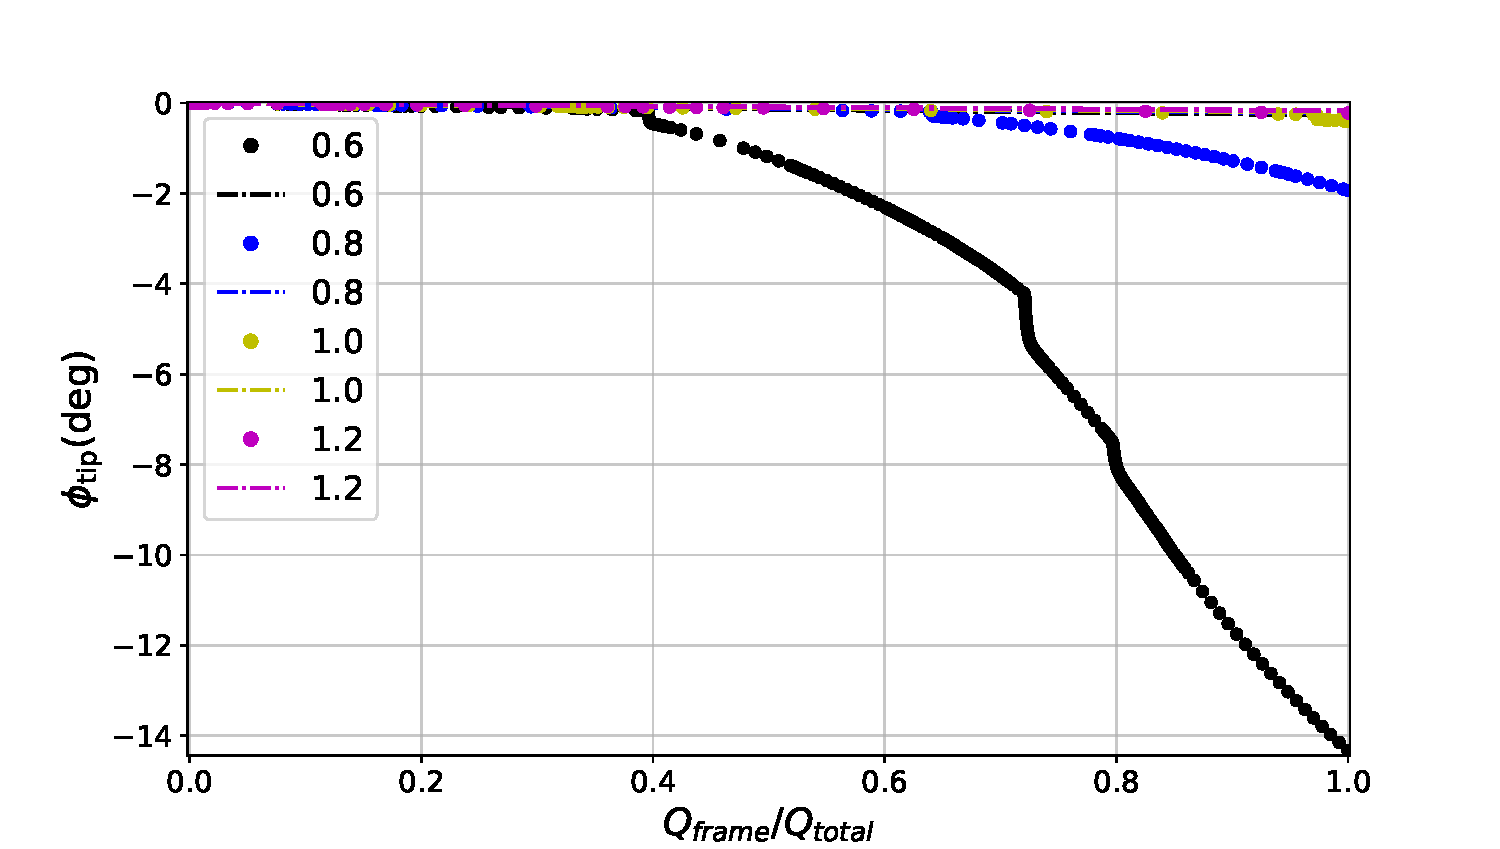
\includegraphics[width=0.8 \textwidth]{../figures/result-sim/cbox/force_displacement-far}
      \caption[Force-displacement curve for various values of the wing-box thickness]{Force-displacement curve for various values of the wing-box thickness \boxt. For all the cases shown, the force applied was located on the upper flange of the tip rib and its magnitude was equal to -800 N.}\label{fig:forceDisplacement-far-Cbox_t}
    \end{figure}

    \begin{figure}[!htpb] %force_displacement-close
      \centering
      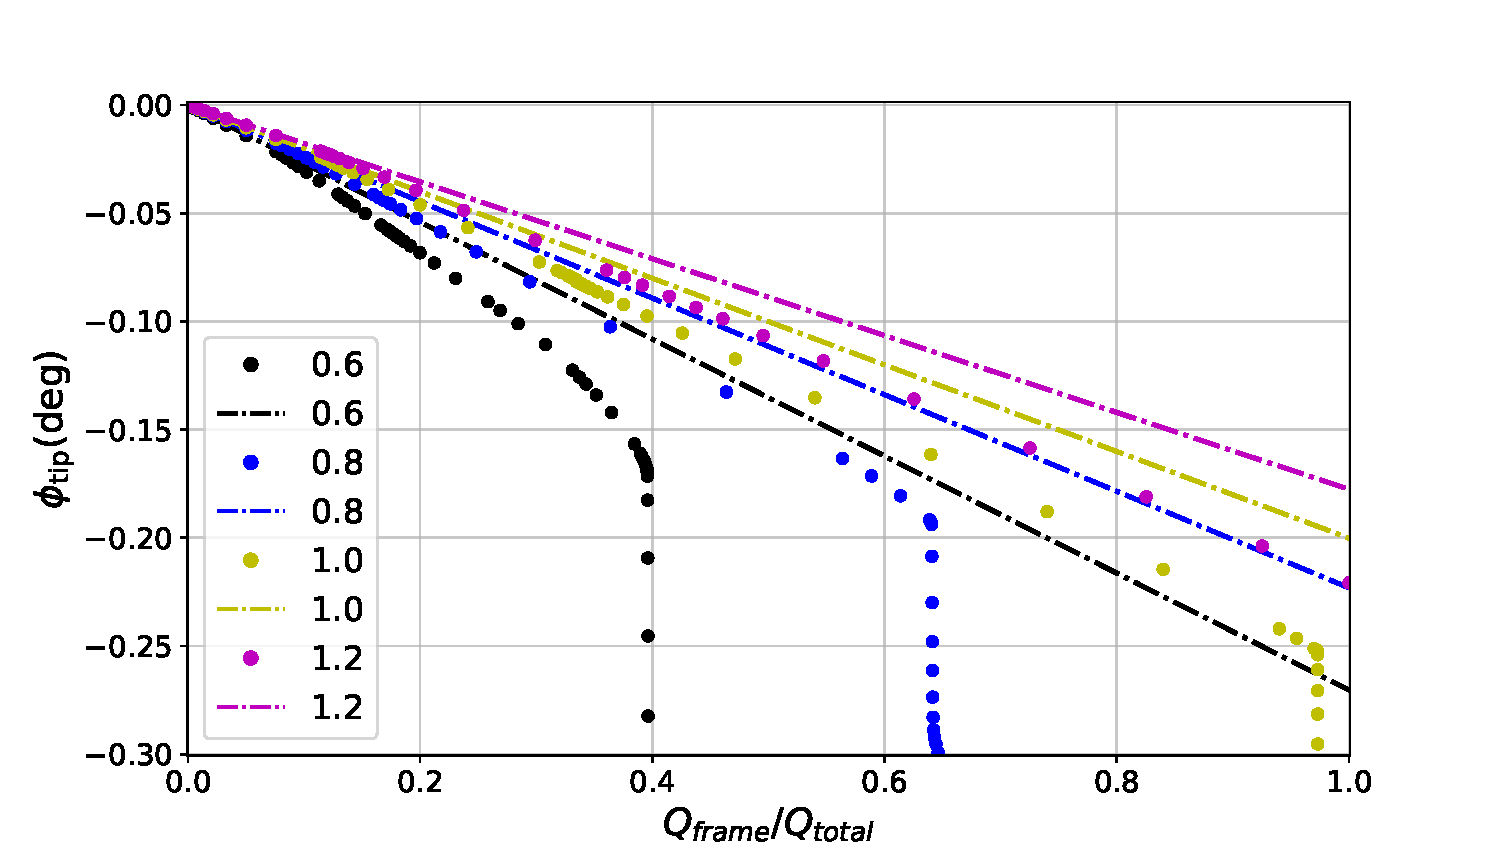
\includegraphics[width=0.8 \textwidth]{../figures/result-sim/cbox/force_displacement-close}
      \caption[Detail of the force-displacement curve for various values of the wing-box thickness]{Detail of the force-displacement curve for various values of the wing-box thickness \boxt. For all the cases shown, the force applied was located on the upper flange of the tip rib and its magnitude was equal to -800 N.}\label{fig:forceDisplacement-close-Cbox_t}
    \end{figure}

    The differences in response for the different cases are also shown the color contour plots provided by Abaqus visualization module. The deformation in the ligaments for \boxt$= 1.2$ mm when buckling occurs is shown in Figure \ref{fig:1coma2-800N-cbox_t} by representing the color contour of the total rotation displacement of the mesh elements. It can be seen buckling does not propagate to other parts of the lattice and it stays where it had appeared on first place, at the first ligaments after the inner rib located further from the root. 

    On the other hand, in Figure \ref{fig:0coma8-800N-cbox_t} the same plot is shown before but not for a value of wing-box thickness of \boxt$= 0.8$ mm. This figure shows the post-buckling state of the structure. In this region, each of the ligaments that had buckled increase its deformation. There are not any new ligaments starting to buckle. It is possible to see that some local deformation has been induced into the upper skin of the wing-box in between the root and the first inner rib. As shown in Table \ref{tab:para_cbox}, for the case $t_{\mathrm{box}} = 0.8$ mm, the point with the maximum vertical is shown to appear close to the root, where $\hat{x}_{v_{\mathrm{max}}} = 0.334$.

    \begin{figure}[!htpb] %force_displacement-close
      \centering
      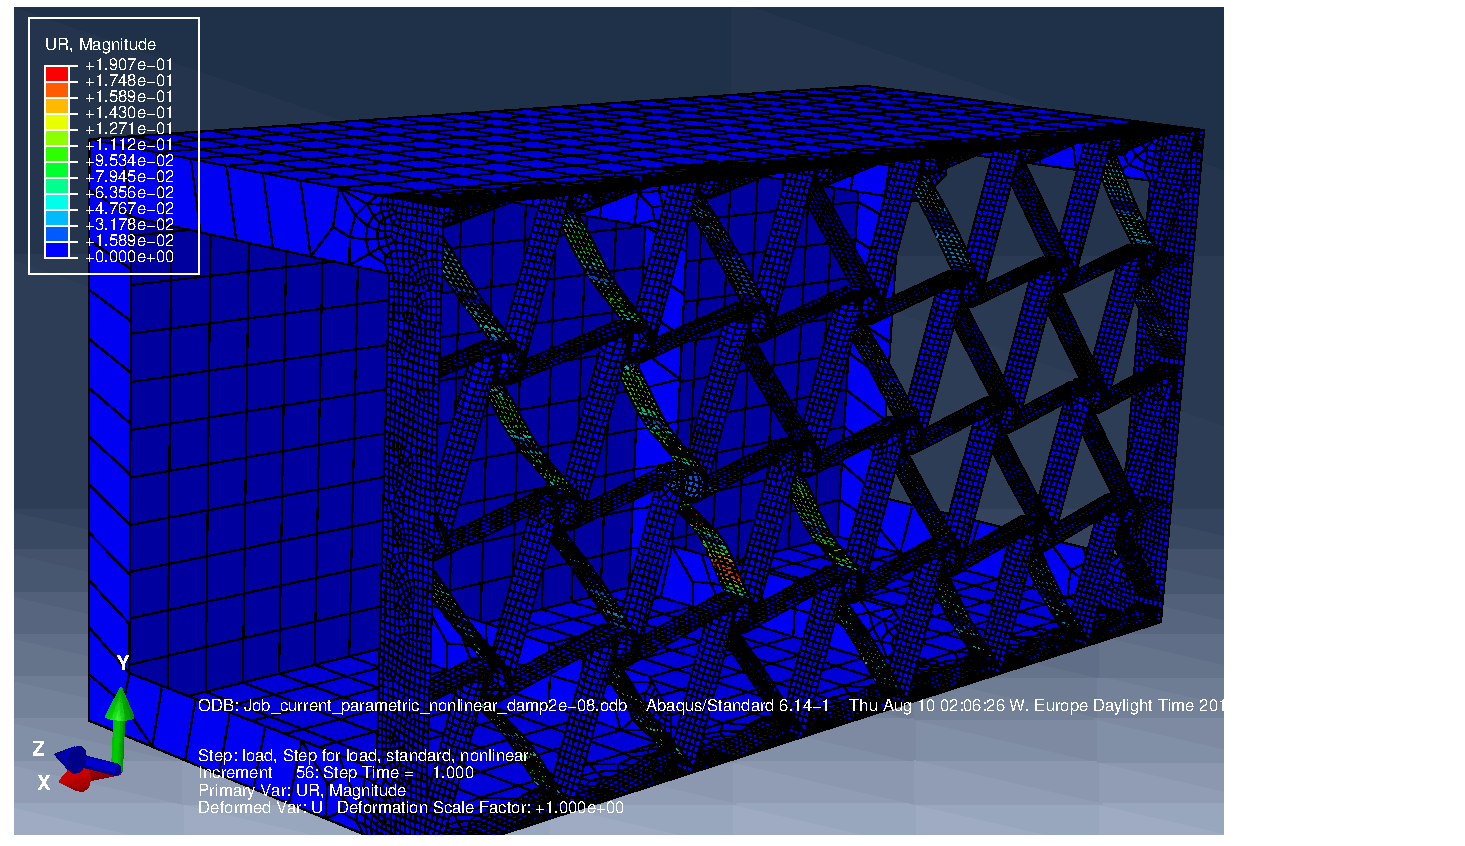
\includegraphics[width=0.8 \textwidth]{../figures/result-sim/cbox/1coma4-800N}
      \caption[Color contour representation of the total angular displacement of the mesh elements on the deformed structure for \boxt$ = 1.2$ mm]{Color contour representation of the total angular displacement of the mesh elements on the deformed structure for \boxt$ = 1.2$ mm. This case is shown after all the prescribed load (800 N) has been applied.}\label{fig:1coma2-800N-cbox_t}
    \end{figure}

    \begin{figure}[!htpb] %force_displacement-close
      \centering
      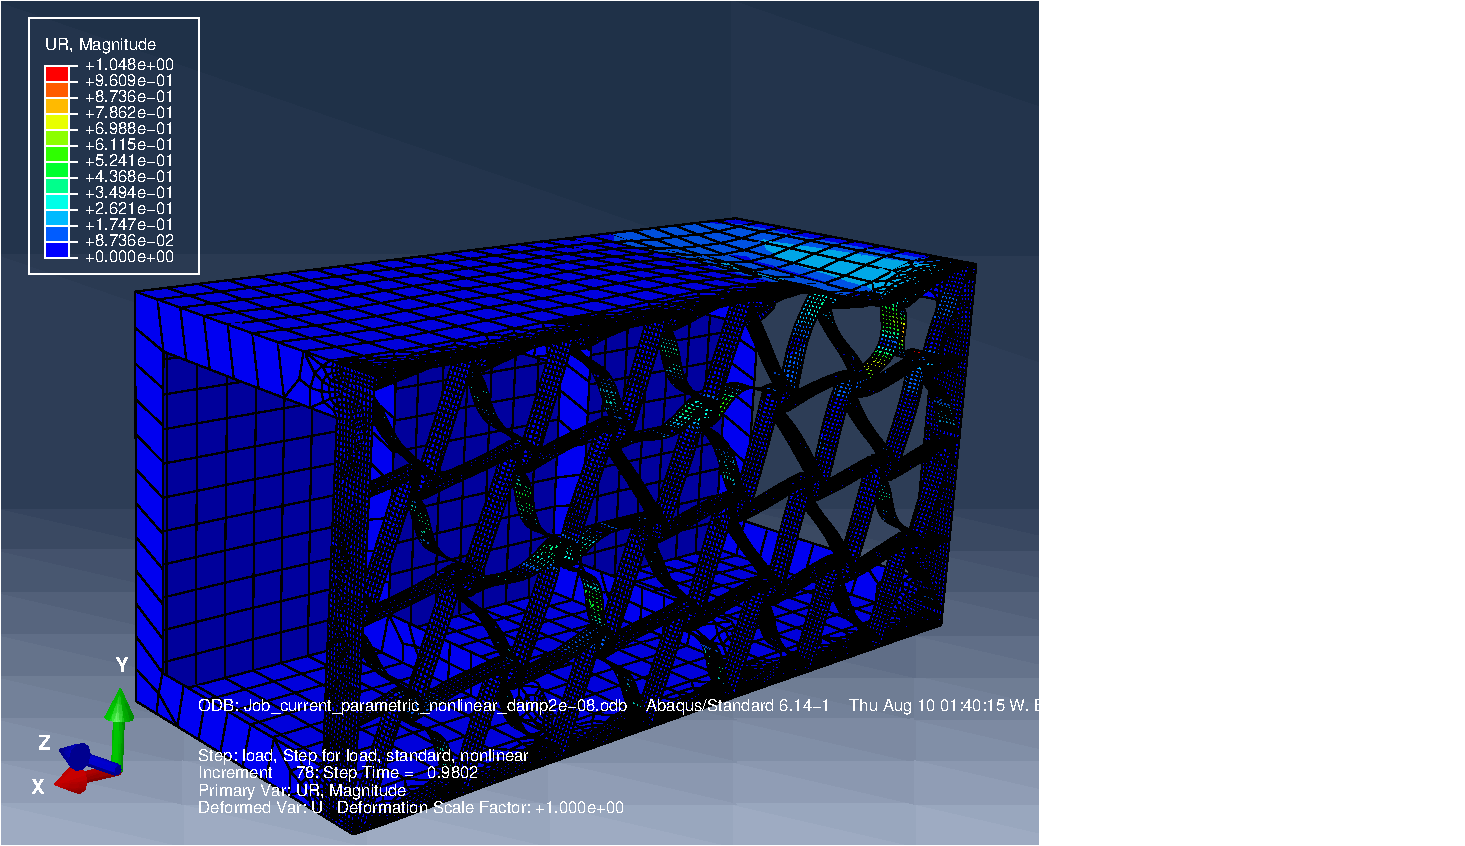
\includegraphics[width=0.8 \textwidth]{../figures/result-sim/cbox/0coma8-800N-2}
      \caption[Color contour representation of the total angular displacement of the mesh elements on the deformed structure for \boxt$ = 0.8$ mm]{Color contour representation of the total angular displacement of the mesh elements on the deformed structure for \boxt$ = 0.8$ mm.}\label{fig:0coma8-800N-cbox_t}
    \end{figure}

    A further study was performed in order to see the relationship between the wing-box thickness and the value of the force applied that induces the structure to collapse. As a result, the plot shown in Figure \ref{fig:force_cbox_t} was produced.

    \begin{figure}[!htpb] %force_plot
      \centering
      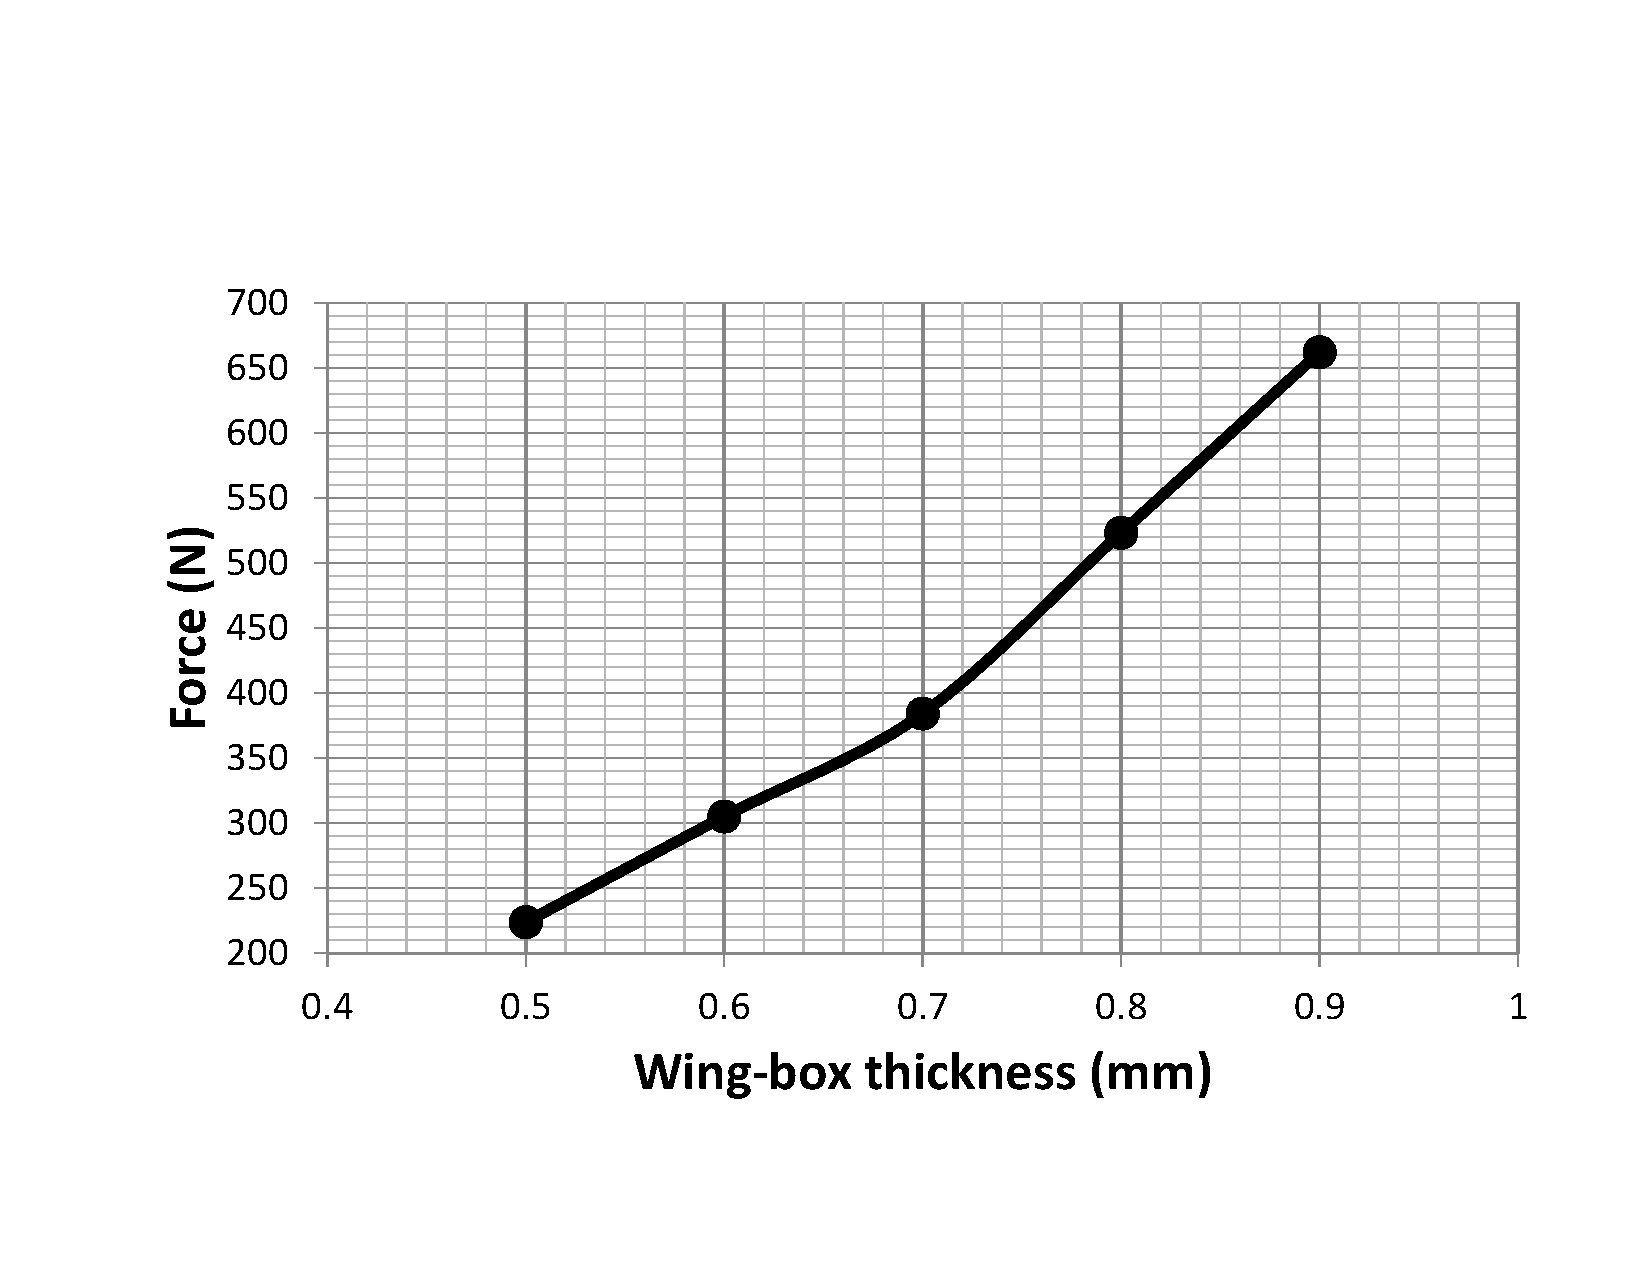
\includegraphics[width=0.8 \textwidth]{../figures/result-sim/cbox/force_cbox_t}
      \caption[Force that induces the structure to collapse as a function of the wing-box thickness]{Force that induces the structure to collapse as a function of the wing-box thickness \boxt.}\label{fig:force_cbox_t}
    \end{figure}

  \clearpage
  \subsection{Number of unit cells in the chiral lattice} \label{subsec:MandN_para}
    %
    %   -> For M:
    %       -It was neccessary to increase the load up to 1200N to see the wing-box with $M = 4$ to collapse

    Now the effect of the number of units cells in the transversal direction $M$ and in the spanwise direction $N$ on the structural response are investigated.

    Firstly, the number of unit cells in the transversal direction $M$ is varied. This parameter modifies the height of the model. Similarly as it was done for the study of the wing-box thickness \boxt influence in the structure response, the results from the different simulations are shown in Table \ref{tab:para_M}. Also, the force-displacement curve is shown in Figure \ref{fig:forceDisplacement-far-M}. It can be seen from results that increments a higher $M$ resulted on a decrement of the structure sensitivity to buckling. For the case of $M = 5$, the structure did not collapse under the prescribed load of 1000 N.

    \begin{table}[!htpb] %Results of M
      \centering
      \begin{tabular}{|l|l|l|l|l|l|l|l|l|}
      \hline
      $M$ & $\phi_{\mathrm{tip}}$ (deg) & $e(\phi_{\mathrm{tip}}) (\%)$ & $\tilde{\phi}_{\mathrm{tip}}$ (deg) & $e(\tilde{\phi}_{\mathrm{tip}}) (\%)$ & $v_{\mathrm{max}}$ & $\hat{z}_{v_{\mathrm{max}}}$ & $\hat{x}_{v_{\mathrm{max}}}$ \\ \hline
      3 & -5.179 & 13.559 & -0.245 & -10.074 & -29.166 & 1 & 0.971 \\ \hline
      4 & -0.392 & 22.16 & -0.148 & -10.447 & -6.093 & 1 & 0.334 \\ \hline
      5 & -0.214 & 14.893 & -0.164 & -17.526 & -1.018 & 0.6 & 0.971 \\ \hline
      \end{tabular}
      \caption[Results from parametric study on the number of unit cells in the transversal direction]{Results from parametric study on the number of unit cells in the transversal direction $M$. The results show the twist at the tip of the wing-box for the Abaqus nonlinear simulation $\phi_{\mathrm{tip}}$ and for the linear simulation $\tilde{\phi}_{\mathrm{tip}}$. The maximum relative error of the mean calculation, expressed as percentage, for these two magnitudes is $e(\phi_{\mathrm{tip}})$ and $e(\tilde{\phi}_{\mathrm{tip}})$, respectively. The table also shows the maximum vertical displacement $v_{\mathrm{max}}$ among all the mesh nodes located on the upper skin of the wing-box and the dimensionless position in the spanwise direction $\hat{x}_{v_{\mathrm{max}}}$ and in the chordwise direction $\hat{z}_{v_{\mathrm{max}}}$ of the node that shows $v = v_{\mathrm{max}}$.}
      \label{tab:para_M}
    \end{table}

    From the results shown in Table \ref{tab:para_B} it can be seen how for the case of $M = 3$, the point that shows $v = v_{\mathrm{max}}$ is located at the wing-box tip where $\hat{x}_{v_{\mathrm{max}}} = 0.971$, due to the high twist of the structure. However, for $M = 4$, the structure has gained stiffness in shear and, even the prescribed load makes the structure to collapse when buckling phenomena appears, the achieved twist $\phi_{\mathrm{tip}}$ is $\approx 7\%$ inferior than what it was obtained for $M = 3$. For $M = 5$, the structure is so stiff that $v_{\mathrm{max}}$ appears approximately at the point where the load is applied. This shows that deformation is only achieved in the vicinity of the load introduction point due to the high stiffness in shear of the structure. 

    \begin{figure}[!htpb] %force_displacement-far
      \centering
      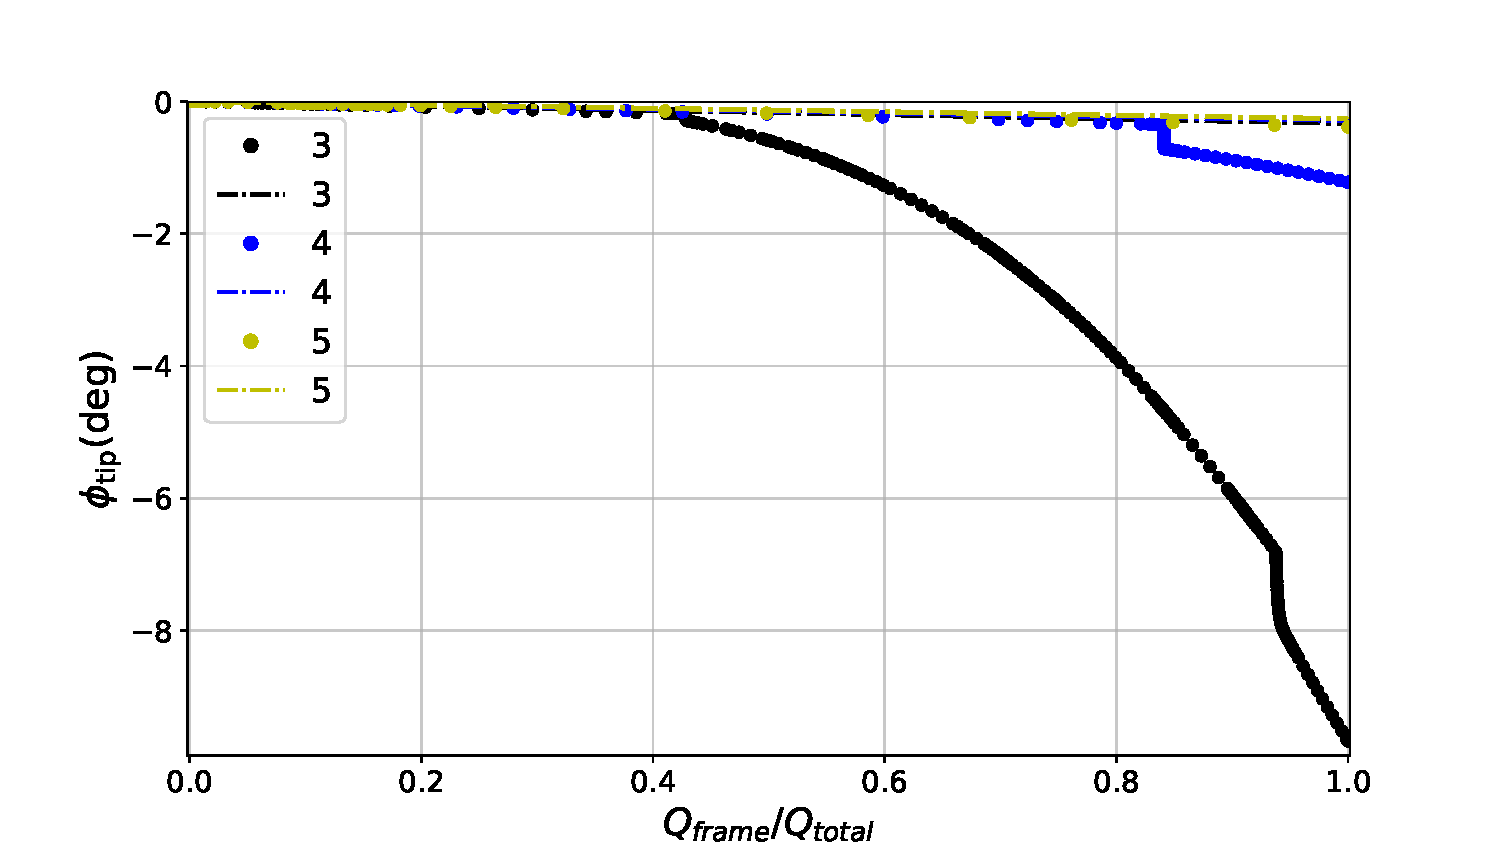
\includegraphics[width=0.8 \textwidth]{../figures/result-sim/M/force_displacement-far-1200N}
      \caption[Force-displacement curve for various values of the number of unit cells in the transversal direction]{Force-displacement curve for various values of the number of unit cells in the transversal direction $M$. For all the cases shown, the load introduction point was located in the middle of the upper flange of the tip rib and its magnitude was equal to -1200 N.}\label{fig:forceDisplacement-far-M}
    \end{figure}

    The effects of the variation of the number of unit cells in the spanwise direction $N$, parameter responsible of the wing-box length is investigated next. The results from the parametric study carried out are shown in Table \ref{tab:para_N}. The force-displacement curve for the simulations carried out is shown in Figure \ref{fig:forceDisplacement-far-N}. It can be seen that the bigger the wing-box length, the earlier that the buckling of the lattices cause the collapse of the structure. 

    %Second stage of the buckling
    In the last plot introduced it can be seen a second change in the slope of the curve for the cases of $N = 10$ and $N = 11$. This happens when, as explained in Section \ref{sec:generalResponseCharact_results_sim}, the buckling phenomena progresses from the ligaments at the root to be more generalized in other parts of the structure. This characteristic can be seen in Figure \ref{fig:N10-UR}, where the response of the structure for the case of $N = 10$ and load fraction of $96\%$ is shown.

    \begin{table}[!htpb] %Results of N
      \centering
      \begin{tabular}{|l|l|l|l|l|l|l|l|l|}
      \hline
      $N$ & $\phi_{\mathrm{tip}}$ (deg) & $e(\phi_{\mathrm{tip}}) (\%)$ & $\tilde{\phi}_{\mathrm{tip}}$ (deg) & $e(\tilde{\phi}_{\mathrm{tip}}) (\%)$ & $v_{\mathrm{max}}$ & $\hat{z}_{v_{\mathrm{max}}}$ & $\hat{x}_{v_{\mathrm{max}}}$ \\ \hline
      7 & -0.185 & 16.474 & -0.14 & -12.506 & -1.061 & 1 & 0.971 \\ \hline
      8 & -0.878 & 9.517 & -0.17 & -10.196 & -9.844 & 1 & 0.334 \\ \hline
      9 & -4.582 & 11.091 & -0.209 & -7.848 & -25.781 & 1 & 0.971 \\ \hline
      10 & -8.116 & 6.192 & -0.248 & -6.398 & -46.636 & 1 & 0.971 \\ \hline
      11 & -17.659 & 4.954 & -0.299 & -5.098 & -107.229 & 1 & 0.971 \\ \hline
      12 & -22.007 & 6.527 & -0.337 & -3.08 & -137.131 & 1 & 0.971 \\ \hline
      \end{tabular}
      \caption[Results from parametric study on the number of unit cells in the spanwise direction]{Results from parametric study on the number of unit cells in the spanwise direction $M$. The results show the twist at the tip of the wing-box for the Abaqus nonlinear simulation $\phi_{\mathrm{tip}}$ and for the linear simulation $\tilde{\phi}_{\mathrm{tip}}$. The maximum relative error of the mean calculation, expressed as percentage, for these two magnitudes is $e(\phi_{\mathrm{tip}})$ and $e(\tilde{\phi}_{\mathrm{tip}})$, respectively. The table also shows the maximum vertical displacement $v_{\mathrm{max}}$ among all the mesh nodes located on the upper skin of the wing-box and the dimensionless position in the spanwise direction $\hat{x}_{v_{\mathrm{max}}}$ and in the chordwise direction $\hat{z}_{v_{\mathrm{max}}}$ of the node that shows $v = v_{\mathrm{max}}$.}
      \label{tab:para_N}
    \end{table}

    \begin{figure}[!htpb] %force_displacement-far
      \centering
      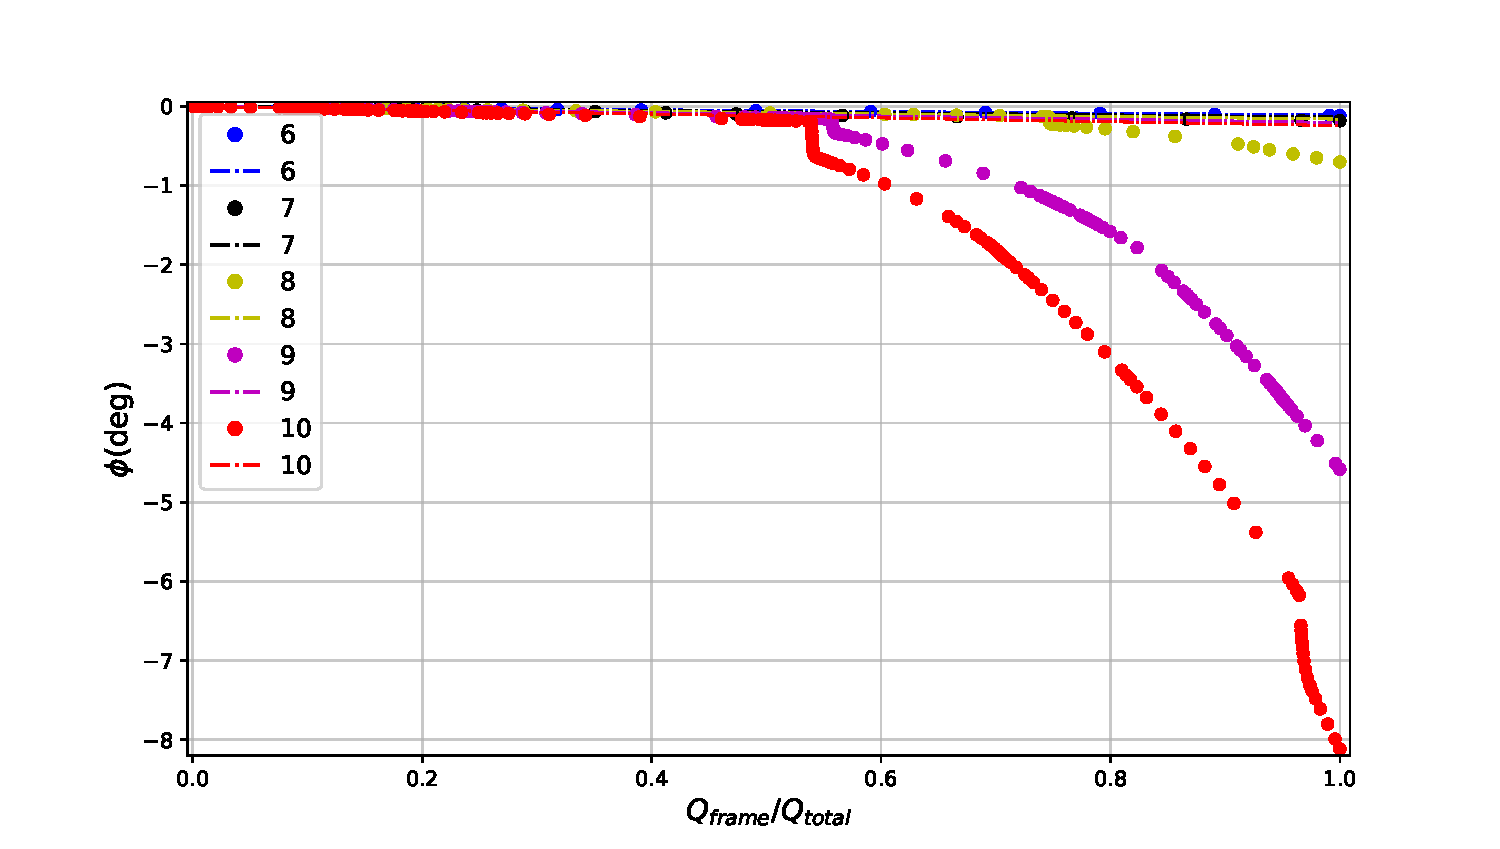
\includegraphics[width=0.8 \textwidth]{../figures/result-sim/N/force_displacement-far}
      \caption[Force-displacement curve for various values of the number of unit cells in the spanwise direction]{Force-displacement curve for various values of the number of unit cells in the spanwise direction $N$. For all the cases shown, the load introduction point was located in the middle of the upper flange of the tip rib and its magnitude was equal to -700 N.}\label{fig:forceDisplacement-far-N}
    \end{figure}

    \begin{figure}[!htpb] %UR for N = 10
      \centering
      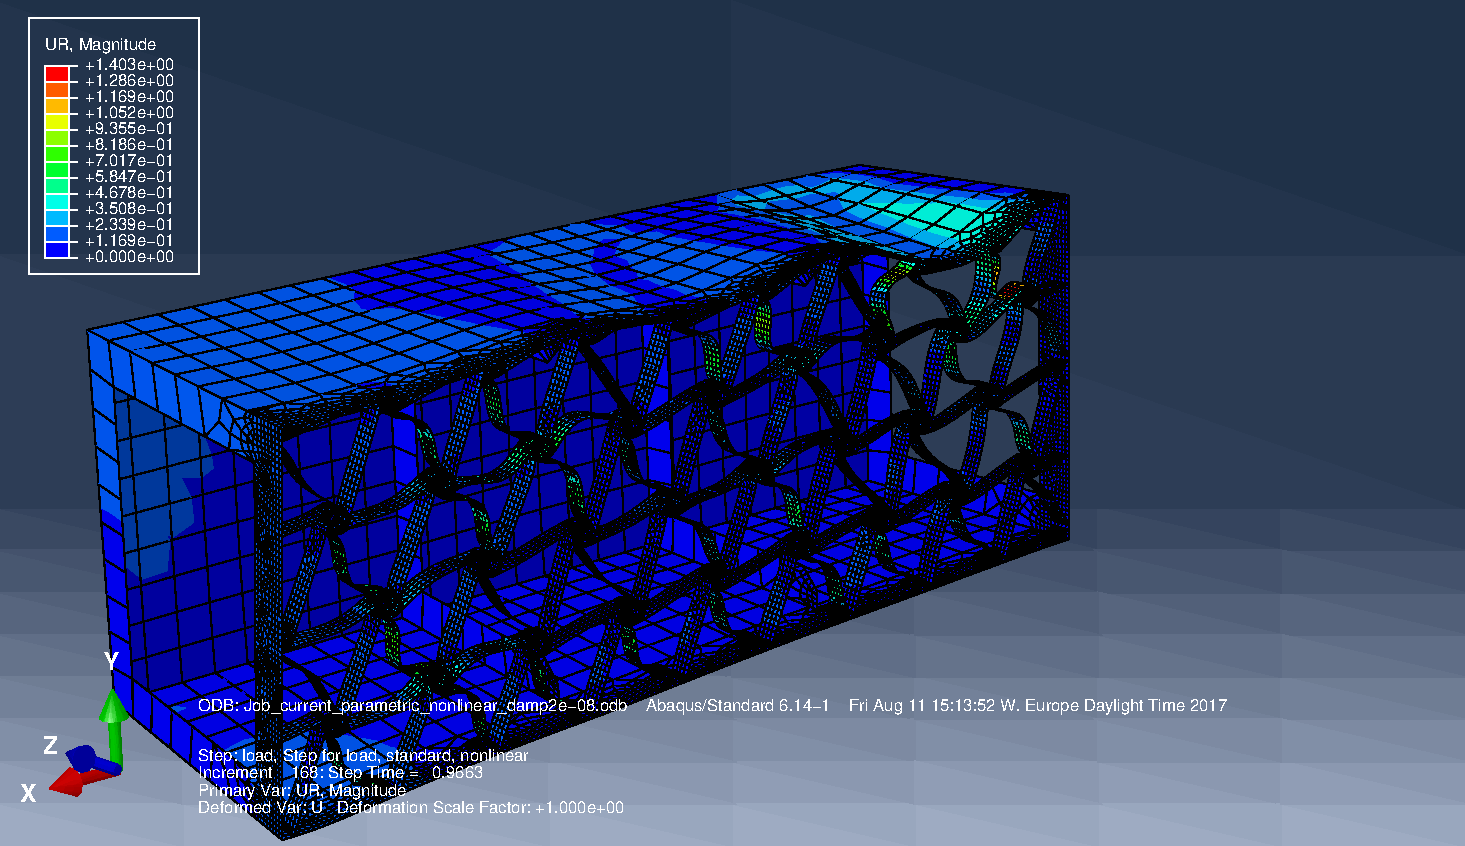
\includegraphics[width=0.8 \textwidth]{../figures/result-sim/N/10}
      \caption[Model response when the fraction of load applied equals to 96\% of the prescribed load (700 N) and $N = 10$]{Model response when the fraction of load applied equals to 96\% of the prescribed load (700 N) and $N = 10$. The plot shows how the buckling phenomena is generalized for the whole chiral structure.}\label{fig:N10-UR}
    \end{figure}

  \clearpage
  \subsection{Chiral lattice parameters} \label{subsec:chiral_para}

    In the present subsection, different parameters of the chiral lattice structure are varied and its effect of the system response are shown. 

    \subsubsection{Dimensionless chiral ligament eccentricity $\hat{e}_{\mathrm{chiral}}$}
      % \ref{fig:../figures/result-sim/eccen/force_displacement-far}
      % In Figure \ref{fig:../figures/result-sim/eccen/0coma1-700N} it can be seen than the excesive eccentricity of the ligaments keep them from causing the collapse of the structure

      The first of the chiral parameter that is going to be studied is the ligament eccentricity $e_{\mathrm{chiral}}$, in its dimensionless form $\hat{e}_{\mathrm{chiral}}$. The numeric results from the simulations carried out can be seen in Table \ref{tab:para_e}.

      The force-deformation curve for the range of simulations carried out can be seen in Figure \ref{fig:forceDisplacement-far-e}. Here it can be seen that the collapse of the structure occurs for all the cases except for \chie$= 0.1$. The deformation state of the structure for this case can be seen in Figure \ref{fig:e0coma1-UR} that shows how the excessive eccentricity of the ligaments keep them from buckling and causing the structure collapse.

      \begin{table}[!htpb] %Results of chiral thickness 
        \centering
        \begin{tabular}{|l|l|l|l|l|l|l|l|l|}
        \hline
        \chie & $\phi_{\mathrm{tip}}$ (deg) & $e(\phi_{\mathrm{tip}}) (\%)$ & $\tilde{\phi}_{\mathrm{tip}}$ (deg) & $e(\tilde{\phi}_{\mathrm{tip}}) (\%)$ & $v_{\mathrm{max}}$ & $\hat{z}_{v_{\mathrm{max}}}$ & $\hat{x}_{v_{\mathrm{max}}}$ \\ \hline
        0.0 & -0.903 & 9.547 & -0.166 & -10.14 & -9.806 & 1 & 0.334 \\ \hline
        0.001 & -1.314 & 13.715 & -0.168 & -9.931 & -12.441 & 1 & 0.334 \\ \hline
        0.01 & -0.877 & 9.525 & -0.17 & -10.196 & -9.831 & 1 & 0.334 \\ \hline
        0.05 & -0.724 & 9.511 & -0.188 & -10.598 & -8.483 & 1 & 0.334 \\ \hline
        0.1 & -0.222 & 9.444 & -0.194 & -10.601 & -1.416 & 1 & 0.971 \\ \hline
        \end{tabular}
        \caption[Results from parametric study on chiral ligament eccentricity]{Results from parametric study on chiral ligament eccentricity \chie. The results show the twist at the tip of the wing-box for the Abaqus nonlinear simulation $\phi_{\mathrm{tip}}$ and for the linear simulation $\tilde{\phi}_{\mathrm{tip}}$. The maximum relative error of the mean calculation, expressed as percentage, for these two magnitudes is $e(\phi_{\mathrm{tip}})$ and $e(\tilde{\phi}_{\mathrm{tip}})$, respectively. The table also shows the maximum vertical displacement $v_{\mathrm{max}}$ among all the mesh nodes located on the upper skin of the wing-box and the dimensionless position in the spanwise direction $\hat{x}_{v_{\mathrm{max}}}$ and in the chordwise direction $\hat{z}_{v_{\mathrm{max}}}$ of the node that shows $v = v_{\mathrm{max}}$.}
        \label{tab:para_e}
      \end{table}

      \begin{figure}[!htpb] %force_displacement-far
        \centering
        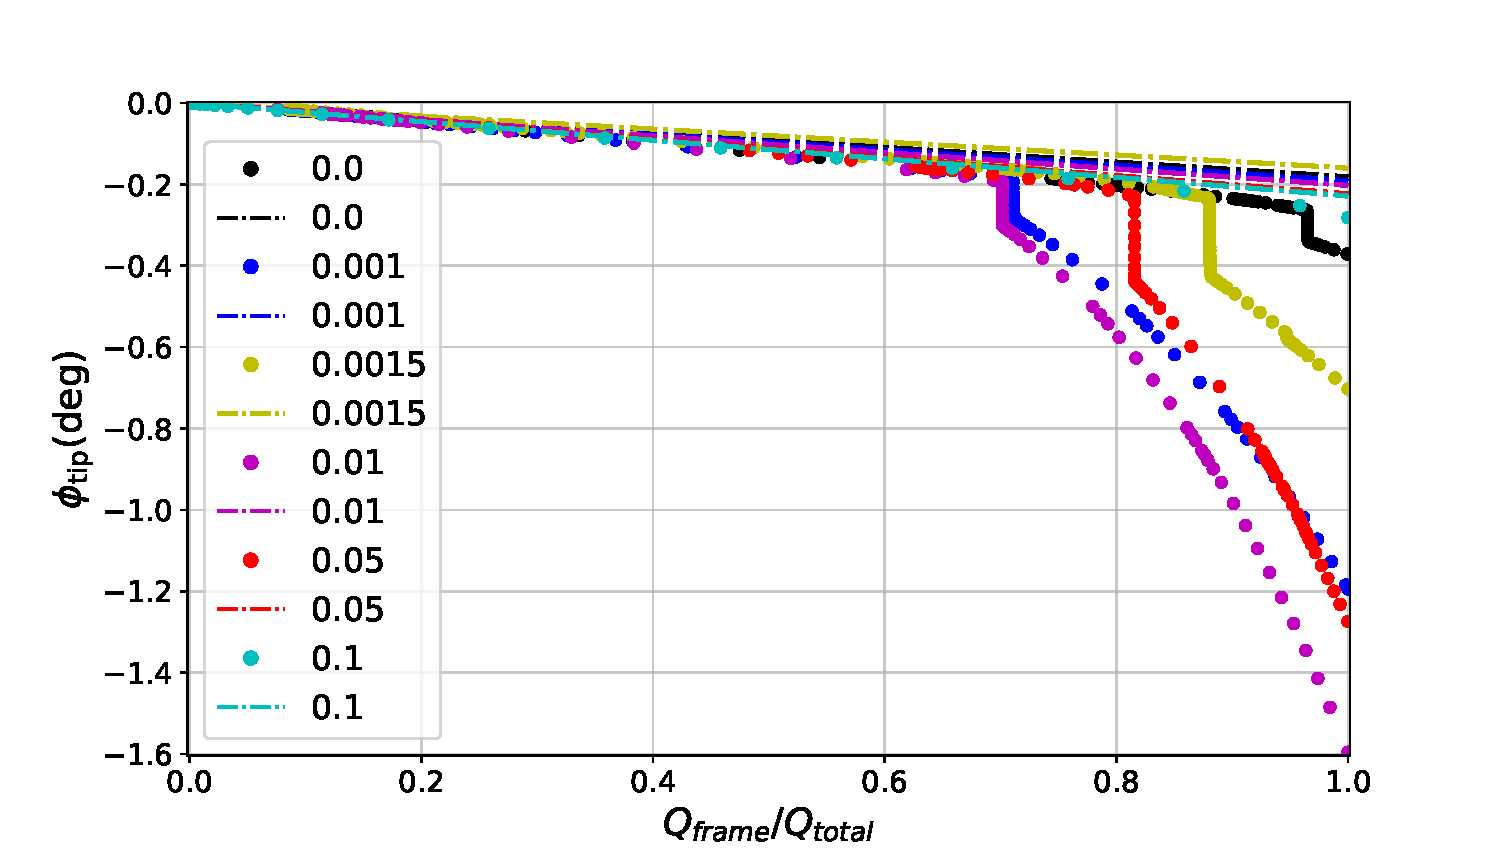
\includegraphics[width=0.8 \textwidth]{../figures/result-sim/eccen/force_displacement-far}
        \caption[Force-displacement curve for various values of the dimensionless chiral ligament eccentricity]{Force-displacement curve for various values of the dimensionless chiral ligament eccentricity \chie. The plot shows how the collapse of the structure occurs for all the cases except for \chie$= 0.1$..}\label{fig:forceDisplacement-far-e}
      \end{figure}

      \begin{figure}[!htpb] %UR for e = 0.1
        \centering
        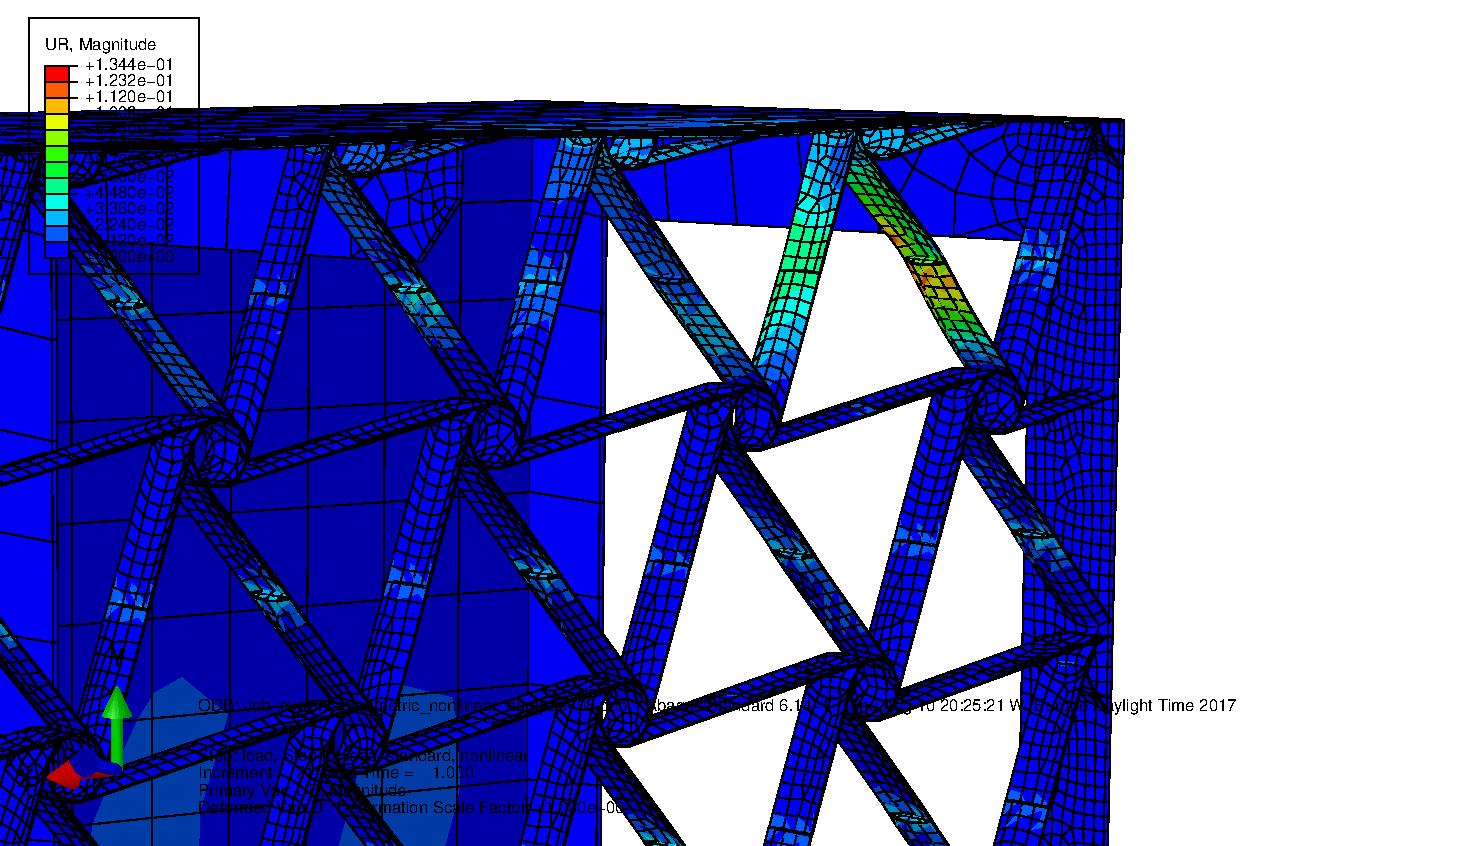
\includegraphics[width=0.8 \textwidth]{../figures/result-sim/eccen/0coma1-700N}
        \caption[Model response when the fraction of load applied equals to 100\% of the prescribed load (700 N) and \chie$= 0.1$]{Model response when the fraction of load applied equals to 100\% of the prescribed load (700 N) and \chie$= 0.1$. For this case, the excessive ligament eccentricity at the end of the simulation keeps it from buckling and causing the structure collapse.}
        \label{fig:e0coma1-UR}
      \end{figure}

      The Figure \ref{fig:forceDisplacement-far-e} also shows that the case of \chie$= 0.0$, that is when the ligaments are flat, is not the case that shows the structure as more sensitive to buckling. Instead, for \chie$= 0.001$ the structure collapses at a smaller load. In other to investigate the load required to make the structure collapse for each particular value of \chit, the plot shown in Figure \ref{fig:force_e} was produced. This shows a minimum for \chie$= 0.001$ showing that different buckling mechanism occurs when the eccentricity is null and when it is not. To investigate this characteristic, the deformed state of the structure is show for \chie$= 0.0$ and \chie$= 0.001$ in Figures \ref{fig:0coma0_UR} and \ref{fig:0coma001_UR}, respectively. This shows effectively, that the buckling mechanism change from case to case. When the eccentricity is null, the structure collapses when buckling appears in two ligaments at the upper part of the root making them to deform and displace the one against the other. However, when the eccentricity is not null, these two ligaments where buckling occurs displace in the same direction towards decreasing values of $x$.

      \begin{figure}[!htpb] %plot with different forces that make the structure to collapse for e
        \centering
        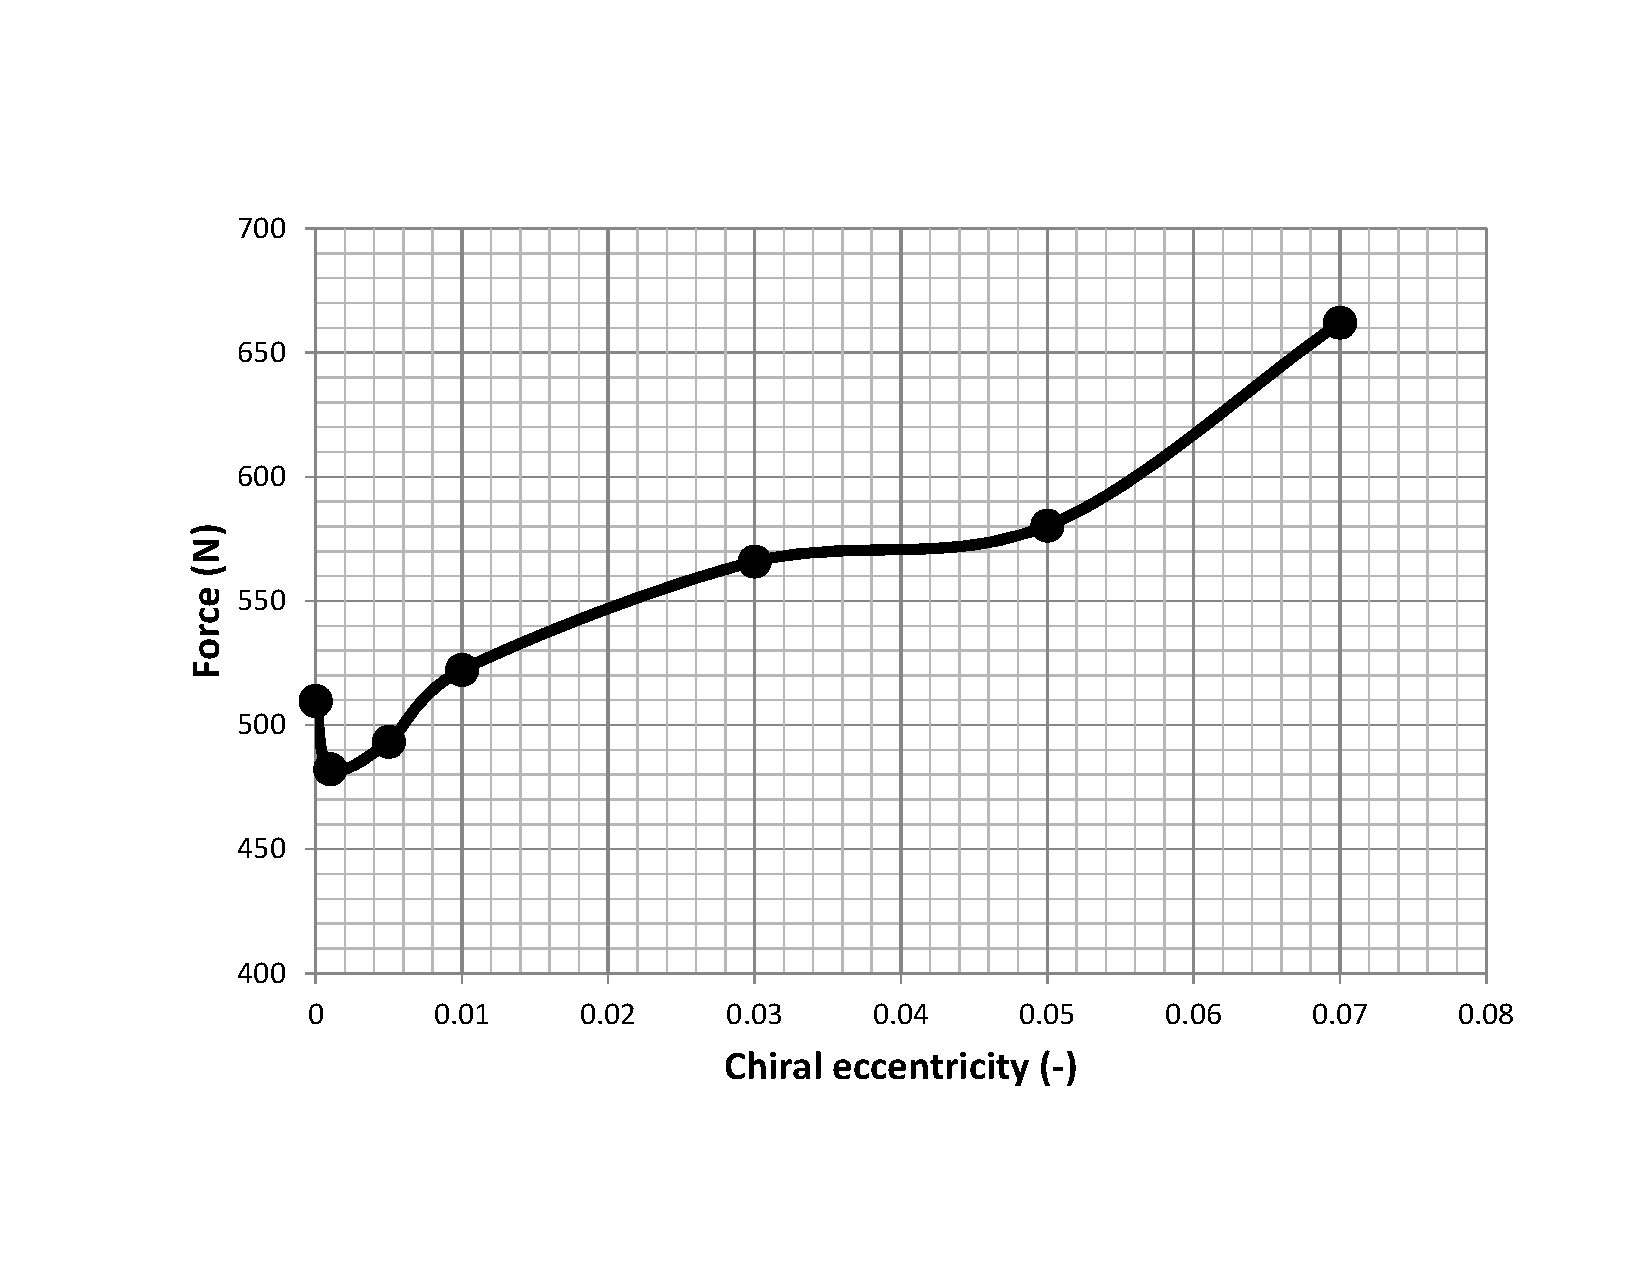
\includegraphics[width=0.8 \textwidth]{../figures/result-sim/eccen/force_e}
        \caption[Force that induces the structure to collapse as a function of the chiral ligament eccentricity]{Force that induces the structure to collapse as a function of the chiral ligament eccentricity \chie. It can be seen that the .}
        \label{fig:force_e}
      \end{figure}

      \begin{figure}[!htpb] %plot with different forces that make the structure to collapse for e
        \centering
        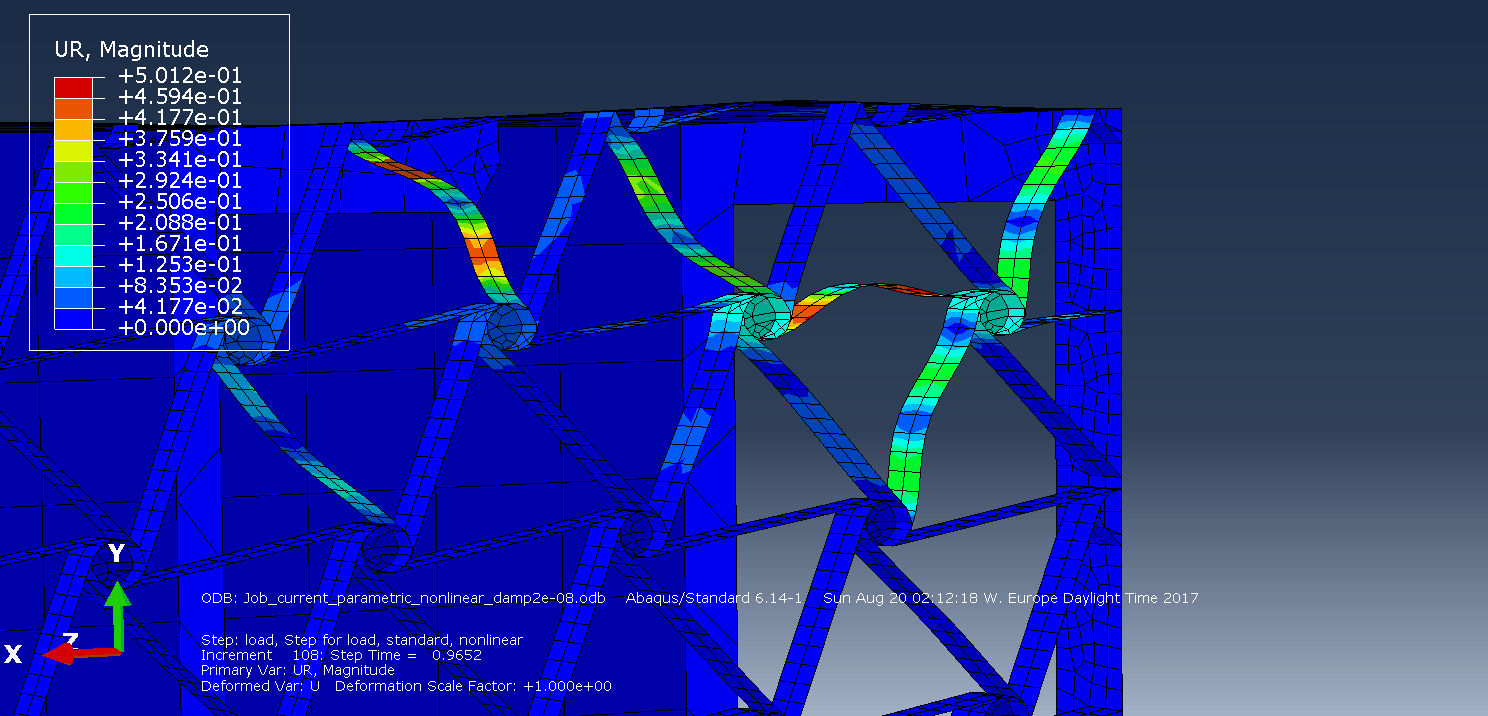
\includegraphics[width=0.8 \textwidth]{../figures/result-sim/eccen/0coma0_UR}
        \caption[Model response when the fraction of load applied equals to 72\% of the prescribed load (700 N) and \chie$= 0.0$]{Model response when the fraction of load applied equals to 72\% of the prescribed load (700 N) and \chie$= 0.0$. For this case, the structure collapse occurs when buckling appears on the ligaments located at the upper part of the root. The deformation makes ligaments to displace the one against each other.}
        \label{fig:0coma0_UR}
      \end{figure}

      \begin{figure}[!htpb] %plot with different forces that make the structure to collapse for e
        \centering
        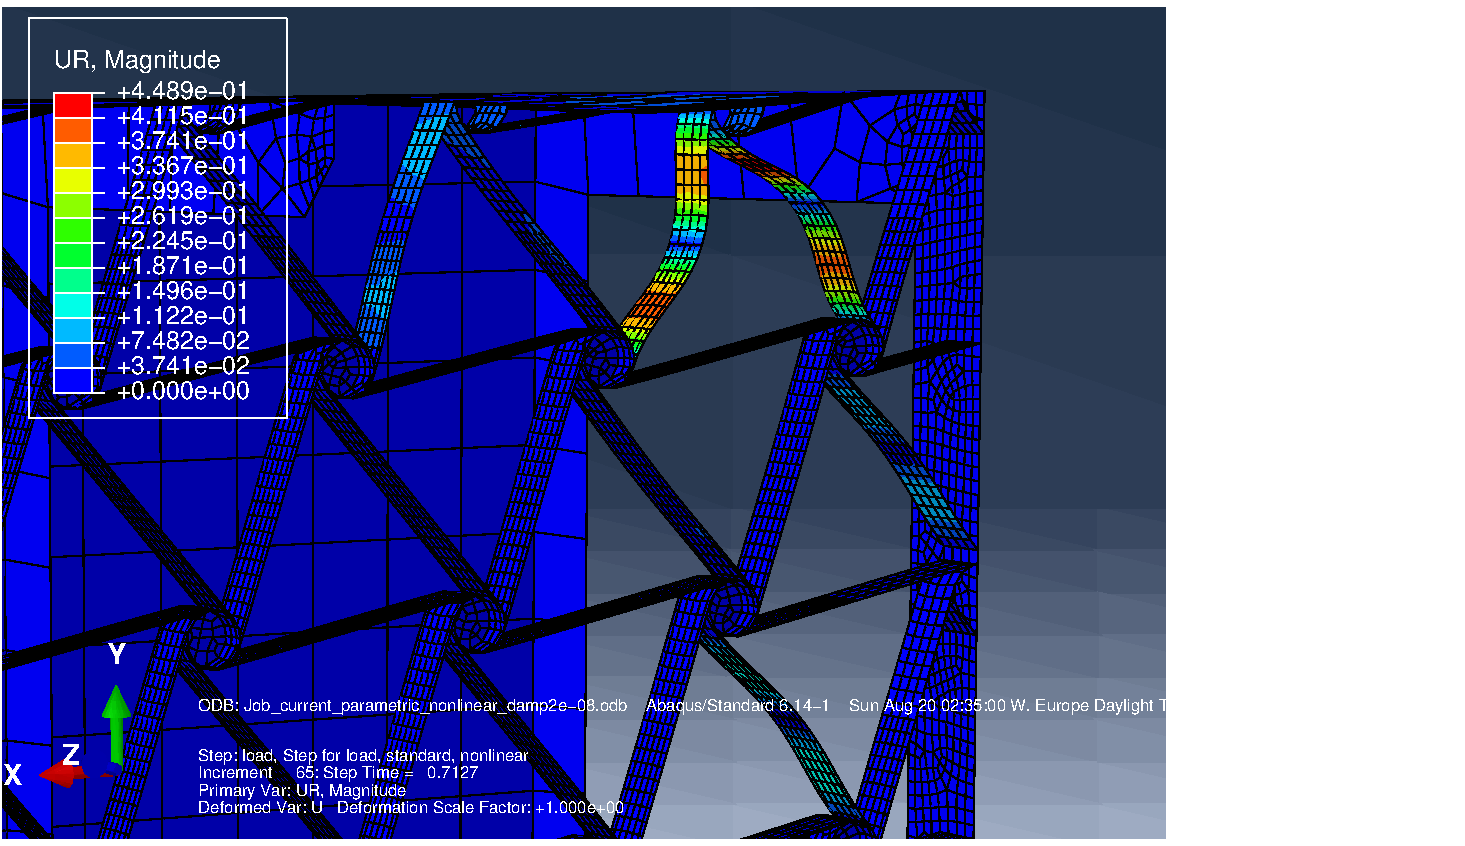
\includegraphics[width=0.8 \textwidth]{../figures/result-sim/eccen/0coma001_UR}
        \caption[Model response when the fraction of load applied equals to 68\% of the prescribed load (700 N) and \chie$= 0.001$]{Model response when the fraction of load applied equals to 68\% of the prescribed load (700 N) and \chie$= 0.001$. For this case, the structure collapse occurs when buckling appears on the ligaments located at the upper part of the root. The deformation makes ligaments to displace in the same direction towards decreasing values of $x$.}
        \label{fig:0coma001_UR}
      \end{figure}


    \clearpage
    \subsubsection{Chiral node depth $B_{\mathrm{chiral}}$}
      %
      % \ref{fig:../figures/result-sim/B/force_displacement-far}
      % The larger the chiral node depth, the bigger surface on the 
      % The collapse point moves backwards as the $B_{\mathrm{chiral}}$ increases. However, the bigger $B_{\mathrm{chiral}}$, the more abrupt the collapse is.
      % It Figure \ref{fig:../figures/result-sim/B/30_UR1} the rotation $UR_1$ of the mesh elements around the $x$ direction can be seen for the case of \B$= 30$mm at the moment when collapse of the structure ocurrs. The value of this magnitude in this area is approximatelly the double to the corresponding one when \B$= 10$mm which can be seen in Figure \ref{fig:../figures/result-sim/B/10_UR1}

      The numeric results from the parametric analysis on the chiral node depth \chiB can be seen in Table \ref{tab:para_B}. The force-displacement curve can be seen in Figure \ref{fig:forceDisplacement-far-B} for various values of $B$. This plot shows how the bigger \chiB is, the more abrupt the collapse is, showing a bigger sudden increment on the measured twist at the tip $\phi_{\mathrm{tip}}$. 

      The Figure \ref{fig:30_UR1} shows the rotation $u$ around the $x$ direction of the mesh elements located on the upper skin of the wing-box and close to the root. This is represented for the case of \chiB$= 30$ mm, at the moment when collapse of the structure occurs which is at $86\%$ of the prescribed load and in the area where local deformation of the skin takes place. Examination of the plot arises that the value of $u$ in this area is approximately double to that corresponding to \chiB$= 10$ mm which can be seen in Figure \ref{fig:10_UR1}. This shows that the bigger \chib is, the more area is affected by the ligaments deformation when buckling occurs and the greater the local deformation will be.

      When plotting the force that makes the structure to collapse against the corresponding value of chiral node depth depth \chiB, the Figure \ref{fig:force_B} was produced.

      \begin{table}[!htpb] %Results of B
        \centering
        \begin{tabular}{|l|l|l|l|l|l|l|l|l|}
        \hline
        \chit & $\phi_{\mathrm{tip}}$ (deg) & $e(\phi_{\mathrm{tip}}) (\%)$ & $\tilde{\phi}_{\mathrm{tip}}$ (deg) & $e(\tilde{\phi}_{\mathrm{tip}}) (\%)$ & $v_{\mathrm{max}}$ & $\hat{z}_{v_{\mathrm{max}}}$ & $\hat{x}_{v_{\mathrm{max}}}$ \\ \hline
        10 & -1.082 & 9.61 & -0.187 & -10.614 & -10.941 & 1 & 0.334 \\ \hline
        20 & -0.877 & 9.525 & -0.17 & -10.196 & -9.831 & 1 & 0.334 \\ \hline
        30 & -0.71 & 9.528 & -0.16 & -9.838 & -8.75 & 1 & 0.334 \\ \hline
        \end{tabular}
        \caption[Results from parametric study on chiral node depth]{Results from parametric study on chiral node depth \chiB. The results show the twist at the tip of the wing-box for the Abaqus nonlinear simulation $\phi_{\mathrm{tip}}$ and for the linear simulation $\tilde{\phi}_{\mathrm{tip}}$. The maximum relative error of the mean calculation, expressed as percentage, for these two magnitudes is $e(\phi_{\mathrm{tip}})$ and $e(\tilde{\phi}_{\mathrm{tip}})$, respectively. The table also shows the maximum vertical displacement $v_{\mathrm{max}}$ among all the mesh nodes located on the upper skin of the wing-box and the dimensionless position in the spanwise direction $\hat{x}_{v_{\mathrm{max}}}$ and in the chordwise direction $\hat{z}_{v_{\mathrm{max}}}$ of the node that shows $v = v_{\mathrm{max}}$.}
        \label{tab:para_B}
      \end{table}

      \begin{figure}[!htpb] %force_displacement-far
        \centering
        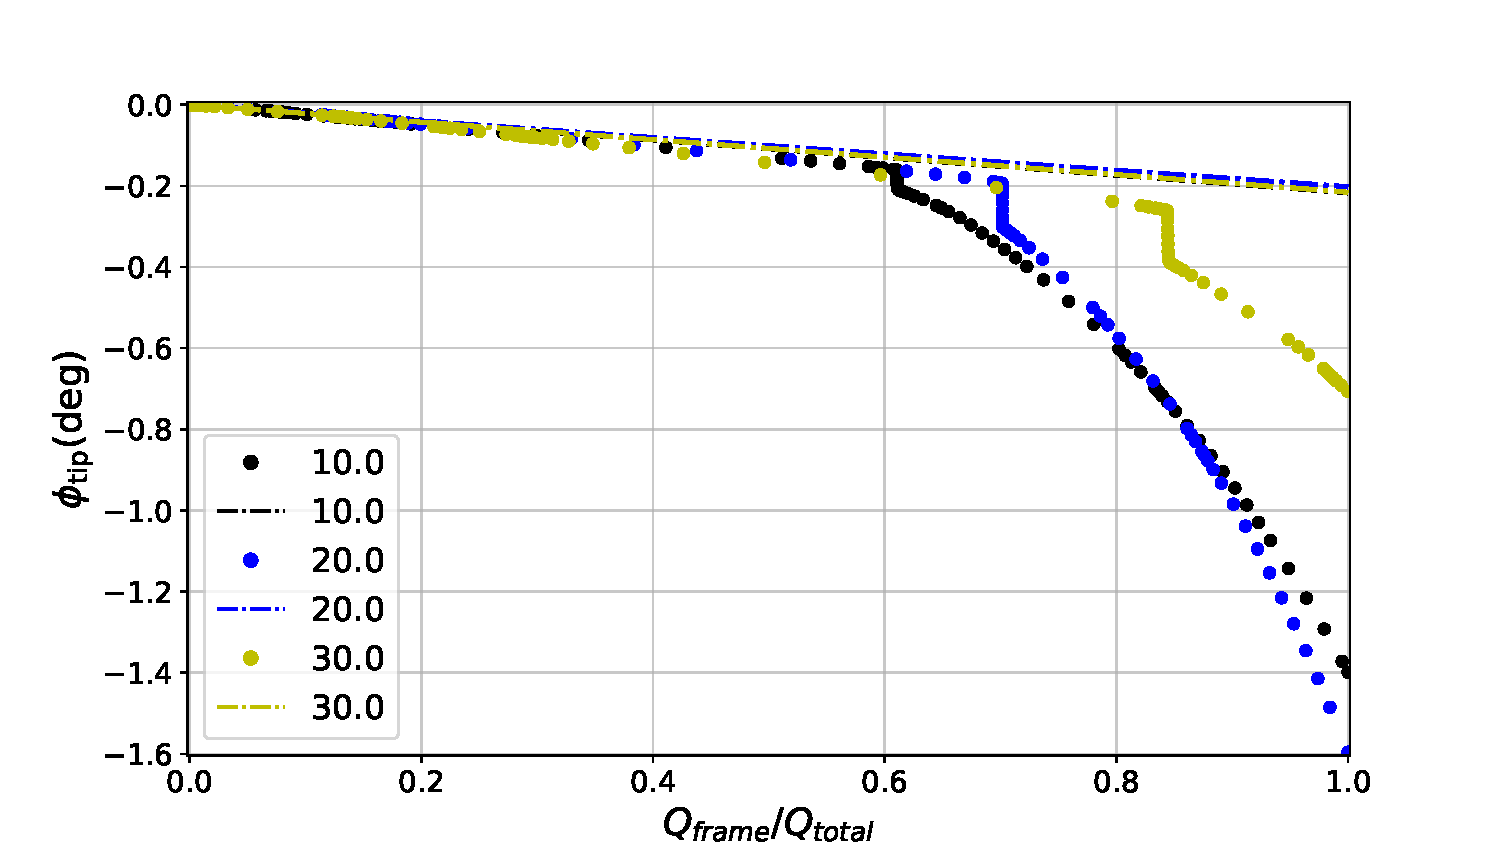
\includegraphics[width=0.8 \textwidth]{../figures/result-sim/B/force_displacement-far}
        \caption[Force-displacement curve for various values of the dimensionless chiral node depth]{Force-displacement curve for various values of the dimensionless chiral node depth \chiB. Results show how the bigger the node depth \chiB is, the later the collapse of the structure occurs but the more abrupt is its.}\label{fig:forceDisplacement-far-B}
      \end{figure}

      \begin{figure}[!htpb] %UR for B = 30
        \centering
        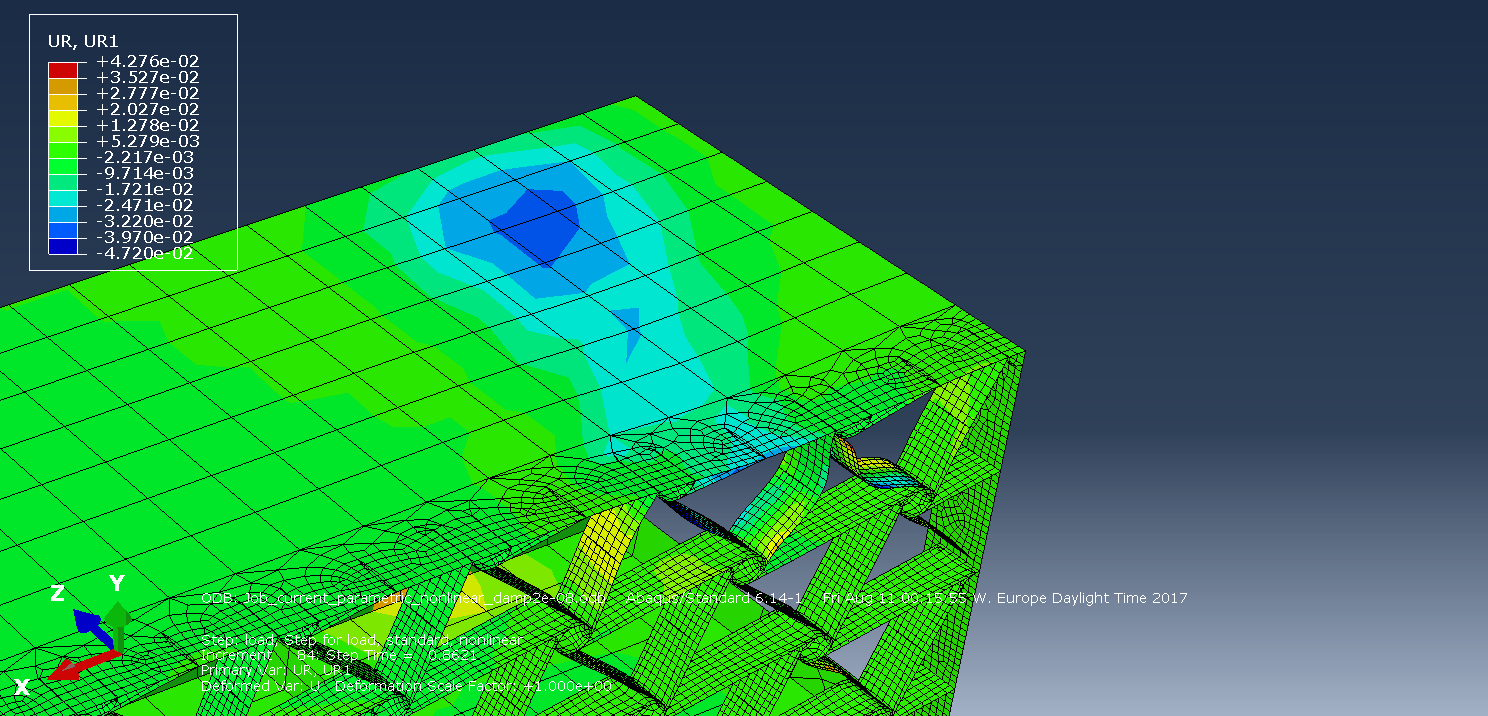
\includegraphics[width=0.8 \textwidth]{../figures/result-sim/B/30_UR1}
        \caption[Model response when the fraction of load applied equals to 86\% of the prescribed load (700 N) and \chiB$= 30$ mm]{Model response when the fraction of load applied equals to 86\% of the prescribed load (700 N) and \chiB$= 30$ mm. The plot shows a color contour with the value of the rotational displacement $u$ around the $x$ direction at the moment in which the structure collapses. In the area where the local deformation occurs, the value of $u$ is approximately equal to $-0.033$ rad.}
        \label{fig:e0coma1-UR}
      \end{figure}

      \begin{figure}[!htpb] %UR for B = 10
        \centering
        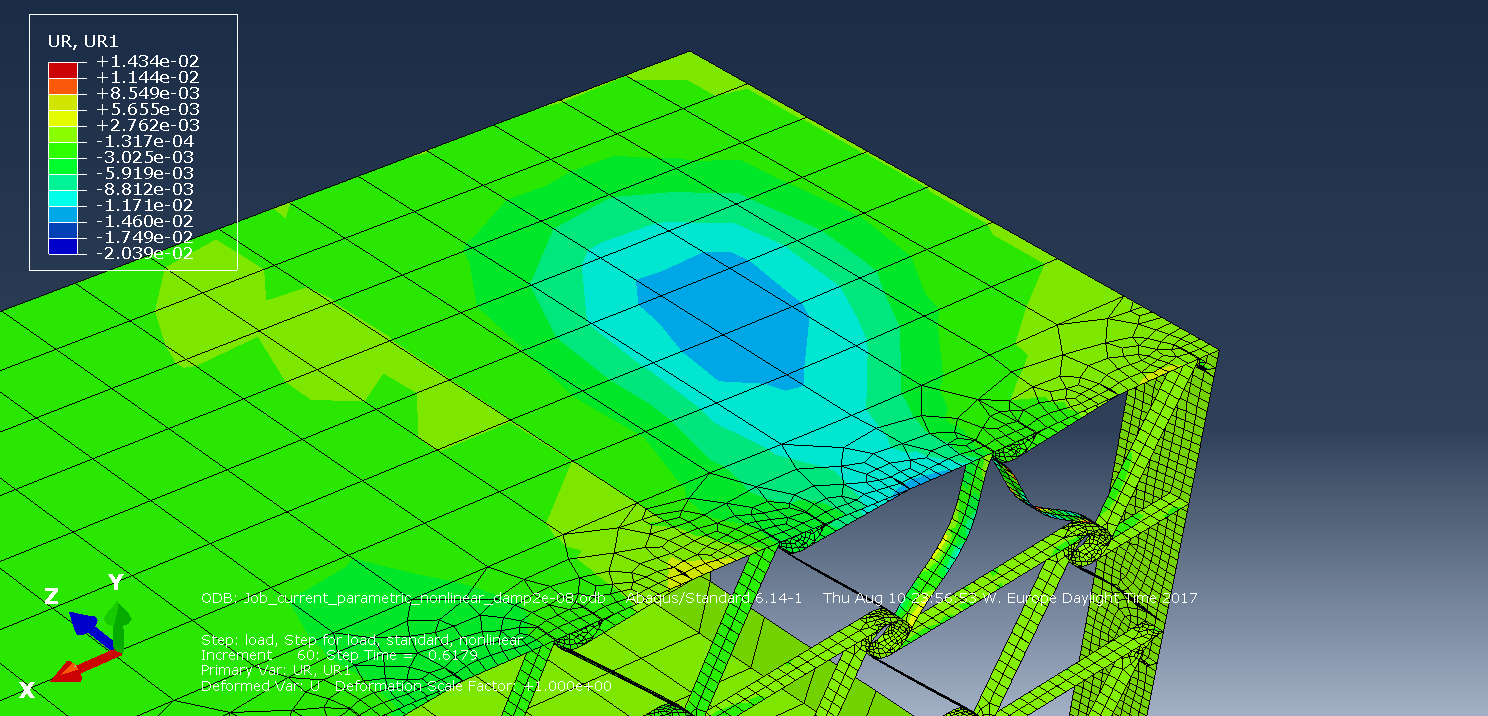
\includegraphics[width=0.8 \textwidth]{../figures/result-sim/B/10_UR1}
        \caption[Model response when the fraction of load applied equals to 62\% of the prescribed load (700 N) and \chiB$= 10$ mm]{Model response when the fraction of load applied equals to 62\% of the prescribed load (700 N) and \chiB$= 10$ mm. The plot shows a color contour with the value of the rotational displacement $u$ around the $x$ direction at the moment in which the structure collapses. In the area where the local deformation occurs, the value of $u$ is approximately equal to $-0.015$ rad.}
        \label{fig:10_UR1}
      \end{figure}

      \begin{figure}[!htpb] %force_plot
        \centering
        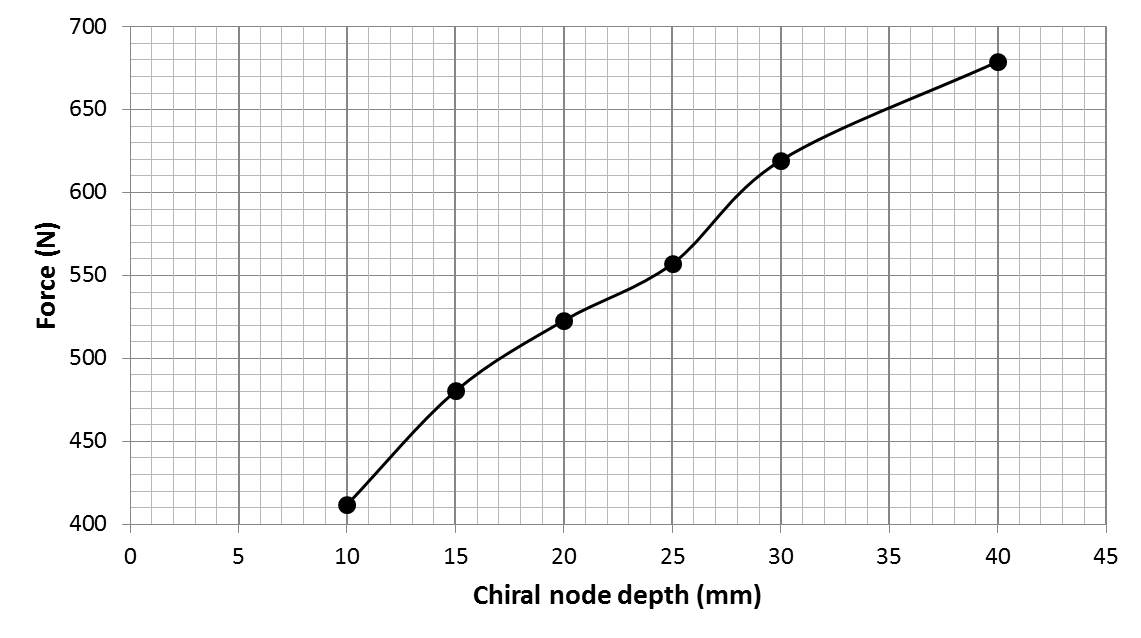
\includegraphics[width=0.8 \textwidth]{../figures/result-sim/B/force_B}
        \caption[Force that induces the structure to collapse as a function of the chiral node depth]{Force that induces the structure to collapse as a function of the chiral node depth \chiB.}\label{fig:force_B}
      \end{figure}

    \clearpage
    \subsubsection{Chiral node radius $r_{\mathrm{chiral}}$}
      %
      % Ranges: 7.5, 10, 12.5, 15, 17.5, 20
      % \ref{fig:../figures/result-sim/r/force_displacement-far}
      % For \r = 5, an error in the ligaments is found. There is interference between the mesh elemnents located at different ligaments that are joined at one node.
      % For \r$= 12.5$mm, the buckling ligaments are located at the root, as it can be seen in Figure \ref{fig:../figures/result-sim/r/12coma5-UR}. However, for the case of \r$= 17.5$mm, buckling do not ocurr on the ligaments located at the root but in those located just after the inner rib located closer to the root, with smaller $x$. This explains the characteristic seen in Figure \ref{fig:../figures/result-sim/r/force_displacement-far} for the case of \r$= 17.5$mm which breaks the trend followed by values \r$< 17.5$mm.

      In the case of the chiral node radius \chir, the possible values were limited by the geometry of the chiral lattice. For values \chir$\le 5$ mm, it was not possible to build the mode due to interferences between the different ligaments that joined at each of the nodes. The numeric results from the simulations are presented in Table \ref{tab:para_r}.

      The force-displacement curve obtained from the simulations is shown in Figure \ref{fig:forceDisplacement-far-r}. This curve shows how the structure collapses for analyzed cases except for \chir$ = 17.5$ mm and \chir$ = 20$ mm. For \chir$= 12.5$mm, the buckling ligaments are located at the root, as it can be seen in Figure \ref{fig:r12coma5-UR}. However, for the case of \chir$= 17.5$mm, buckling do not occur on the ligaments located at the root but in those located just after the inner rib located closer to the root, with smaller $x$. This explains the characteristic seen in Figure \ref{fig:../figures/result-sim/r/force_displacement-far} for the case of \chir$= 17.5$mm which breaks the trend followed by values \chir$< 17.5$mm. Then, the chiral node radius \chir value shifts the position of the buckling ligaments that origin the collapse of the structure.

      The variation of the force that makes the structure to collapse as a function of the chiral node radius \chir can be seen in Figure \ref{fig:force_r}.

      \begin{table}[!htpb] %Results of r
        \centering
        \begin{tabular}{|l|l|l|l|l|l|l|l|l|}
        \hline
        \chir & $\phi_{\mathrm{tip}}$ (deg) & $e(\phi_{\mathrm{tip}}) (\%)$ & $\tilde{\phi}_{\mathrm{tip}}$ (deg) & $e(\tilde{\phi}_{\mathrm{tip}}) (\%)$ & $v_{\mathrm{max}}$ & $\hat{z}_{v_{\mathrm{max}}}$ & $\hat{x}_{v_{\mathrm{max}}}$ \\ \hline
        7.5 & -1.184 & 13.64 & -0.171 & -10.046 & -11.586 & 1 & 0.331 \\ \hline
        10 & -0.877 & 9.525 & -0.17 & -10.196 & -9.831 & 1 & 0.334 \\ \hline
        12.5 & -0.886 & 9.596 & -0.17 & -10.247 & -10.051 & 1 & 0.337 \\ \hline
        15 & -1.121 & 13.638 & -0.173 & -10.134 & -11.677 & 1 & 0.342 \\ \hline
        17.5 & -0.273 & 9.481 & -0.171 & -10.215 & -4.169 & 1 & 0.568 \\ \hline
        20 & -0.229 & 12.686 & -0.171 & -8.848 & -1.433 & 1 & 1.026 \\ \hline
        \end{tabular}
        \caption[Results from parametric study on chiral node radius]{Results from parametric study on chiral node radius \chir. The results show the twist at the tip of the wing-box for the Abaqus nonlinear simulation $\phi_{\mathrm{tip}}$ and for the linear simulation $\tilde{\phi}_{\mathrm{tip}}$. The maximum relative error of the mean calculation, expressed as percentage, for these two magnitudes is $e(\phi_{\mathrm{tip}})$ and $e(\tilde{\phi}_{\mathrm{tip}})$, respectively. The table also shows the maximum vertical displacement $v_{\mathrm{max}}$ among all the mesh nodes located on the upper skin of the wing-box and the dimensionless position in the spanwise direction $\hat{x}_{v_{\mathrm{max}}}$ and in the chordwise direction $\hat{z}_{v_{\mathrm{max}}}$ of the node that shows $v = v_{\mathrm{max}}$.}
        \label{tab:para_r}
      \end{table}

      \begin{figure}[!htpb] %force_displacement-far
        \centering
        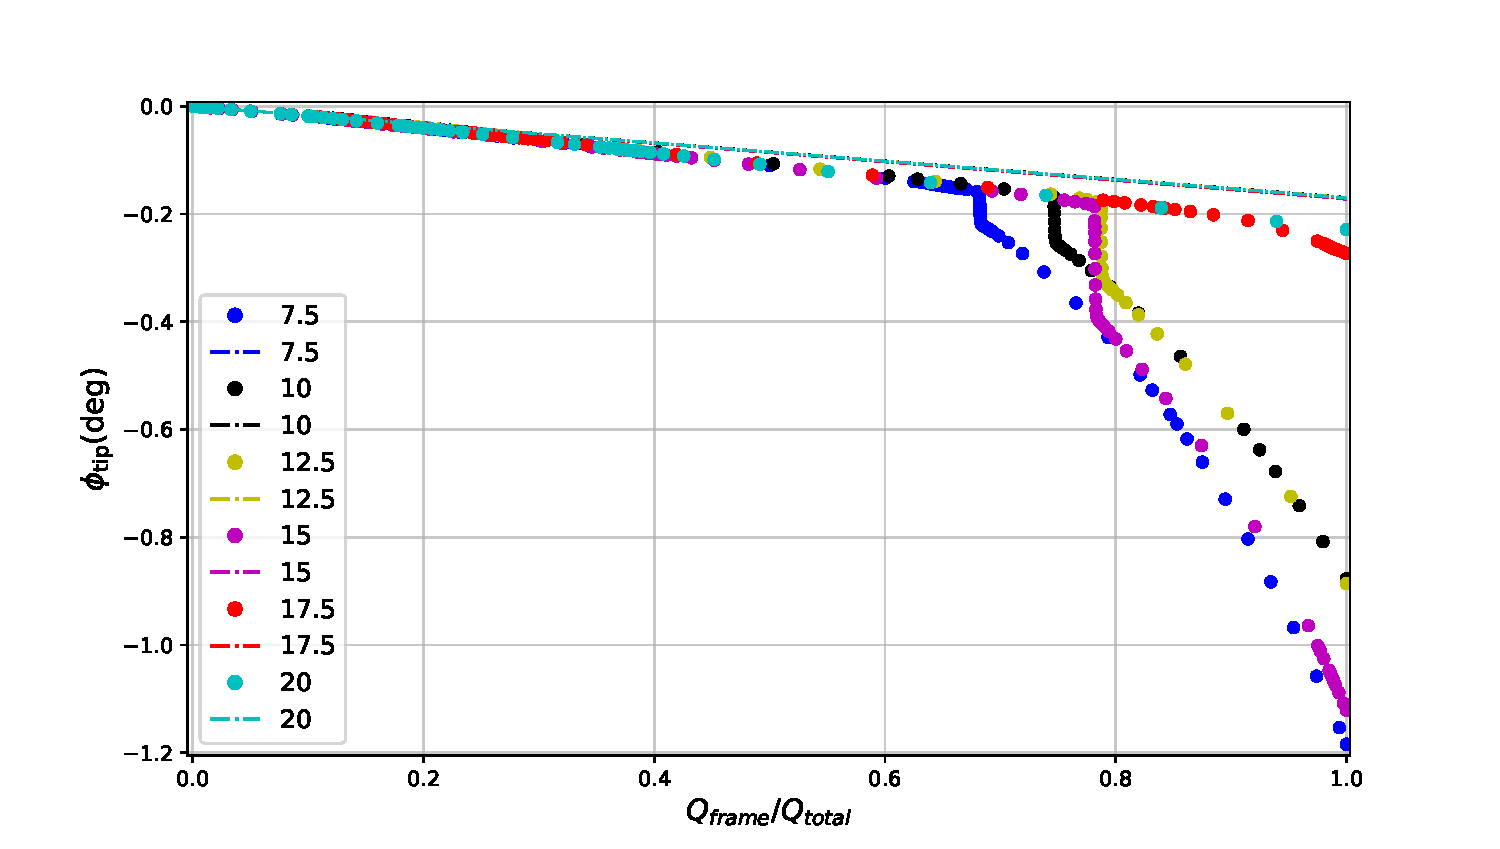
\includegraphics[width=0.8 \textwidth]{../figures/result-sim/r/force_displacement-far}
        \caption[Force-displacement curve for various values of the chiral node radius]{Force-displacement curve for various values of the chiral node radius \chir.}\label{fig:forceDisplacement-far-r}
      \end{figure}

      \begin{figure}[!htpb] %UR for r = 12.5
        \centering
        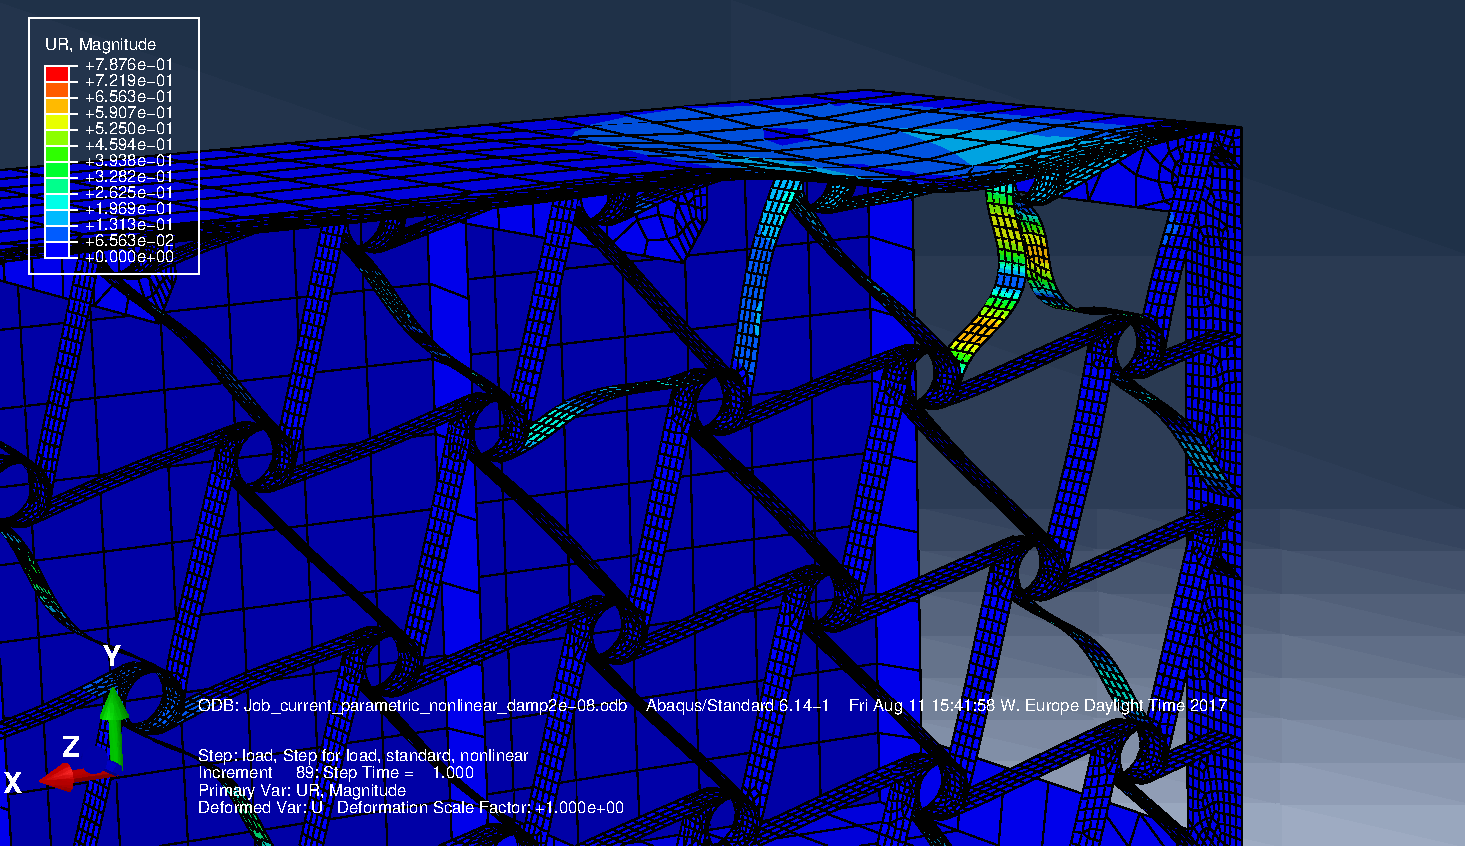
\includegraphics[width=0.8 \textwidth]{../figures/result-sim/r/12coma5-UR}
        \caption[Model response when the fraction of load applied equals to 100\% of the prescribed load (700 N) and \chir$ = 12.5$ mm]{Model response when the fraction of load applied equals to 100\% of the prescribed load (700 N) and \chir$ = 12.5$ mm. Results show that buckling occurs here for ligaments located at the root, as shown in for the baseline configuration.}\label{fig:r12coma5-UR}
      \end{figure}

      \begin{figure}[!htpb] %UR for r = 17.5
        \centering
        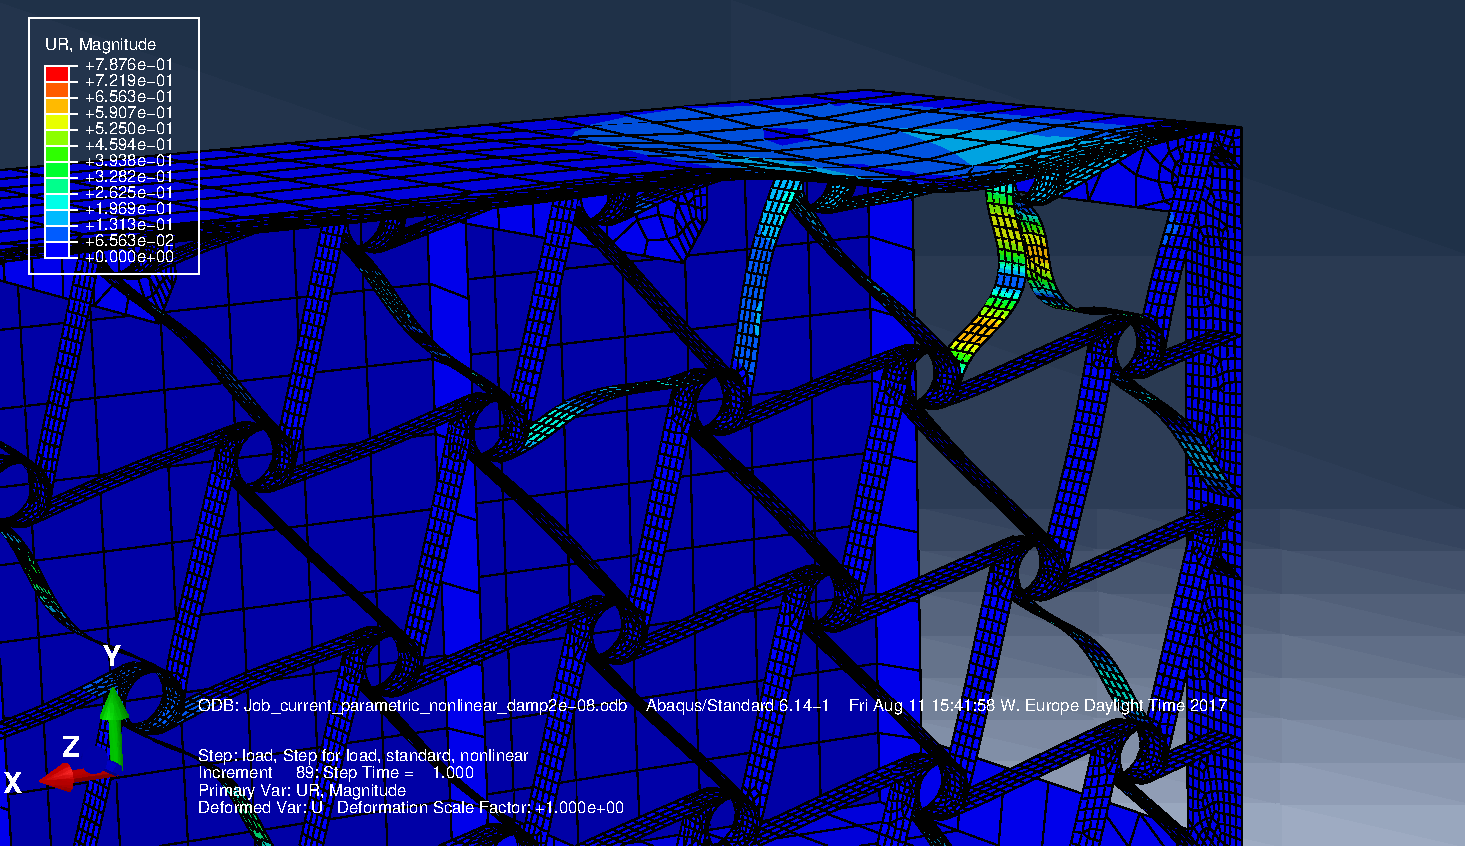
\includegraphics[width=0.8 \textwidth]{../figures/result-sim/r/12coma5-UR}
        \caption[Model response when the fraction of load applied equals to 100\% of the prescribed load (700 N) and \chir$ = 17.5$ mm]{Model response when the fraction of load applied equals to 100\% of the prescribed load (700 N) and \chir$ = 17.5$ mm. Here, the excessive value of }\label{fig:r17coma5-UR}
      \end{figure}

      \begin{figure}[!htpb] %force_plot
        \centering
        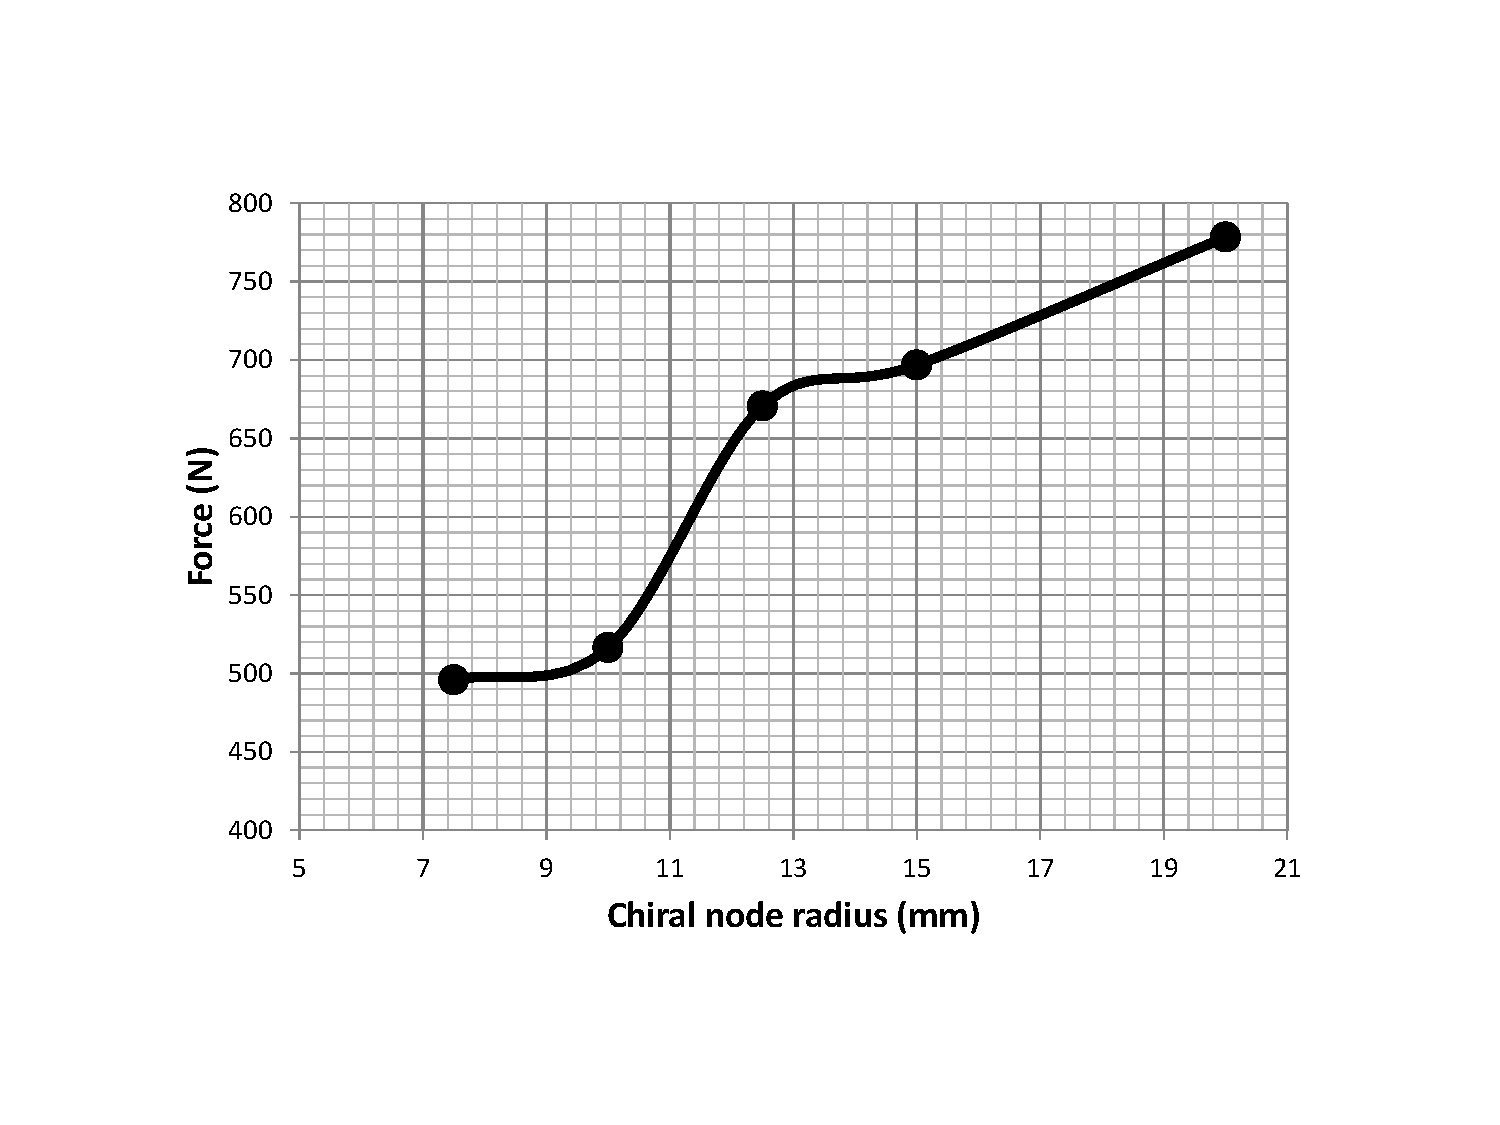
\includegraphics[width=0.8 \textwidth]{../figures/result-sim/r/force_r}
        \caption[Force that induces the structure to collapse as a function of the chiral node depth]{Force that induces the structure to collapse as a function of the chiral node radius \chir.}\label{fig:force_r}
      \end{figure}

    \subsubsection{Chiral ligament half length $L_{\mathrm{chiral}}$}
      %
      %

      The numeric results obtained for the parametric study on the chiral ligament half length \chiL are shown in Table \ref{tab:para_L}. The force-displacement curve for the set of values analysed is shown in Figure \ref{fig:forceDisplacement-far-L}. This plot shows that the bigger the ligament half length is, the earlier that the structure will collapse after severe buckling of the ligaments at the root. For the case of \chiL$= 30$, the structure does not collapse as the structure has become very stiff.    

      \begin{table}[!htpb] %Results of L
        \centering
        \begin{tabular}{|l|l|l|l|l|l|l|l|l|}
        \hline
        \chiL & $\phi_{\mathrm{tip}}$ (deg) & $e(\phi_{\mathrm{tip}}) (\%)$ & $\tilde{\phi}_{\mathrm{tip}}$ (deg) & $e(\tilde{\phi}_{\mathrm{tip}}) (\%)$ & $v_{\mathrm{max}}$ & $\hat{z}_{v_{\mathrm{max}}}$ & $\hat{x}_{v_{\mathrm{max}}}$ \\ \hline
        30 & -0.162 & 11.739 & -0.124 & -9.441 & -1.032 & 1 & 0.602 \\ \hline
        50 & -0.877 & 9.525 & -0.170 & -10.196 & -9.831 & 1 & 0.334 \\ \hline
        70 & -4.374 & 8.563 & -0.205 & -9.915 & -27.936 & 1 & 0.463 \\ \hline
        \end{tabular}
        \caption[Results from parametric study on chiral ligament half length]{Results from parametric study on chiral ligament half length \chir. The results show the twist at the tip of the wing-box for the Abaqus nonlinear simulation $\phi_{\mathrm{tip}}$ and for the linear simulation $\tilde{\phi}_{\mathrm{tip}}$. The maximum relative error of the mean calculation, expressed as percentage, for these two magnitudes is $e(\phi_{\mathrm{tip}})$ and $e(\tilde{\phi}_{\mathrm{tip}})$, respectively. The table also shows the maximum vertical displacement $v_{\mathrm{max}}$ among all the mesh nodes located on the upper skin of the wing-box and the dimensionless position in the spanwise direction $\hat{x}_{v_{\mathrm{max}}}$ and in the chordwise direction $\hat{z}_{v_{\mathrm{max}}}$ of the node that shows $v = v_{\mathrm{max}}$.}
        \label{tab:para_L}
      \end{table}

      \begin{figure}[!htpb] %force_displacement-far
        \centering
        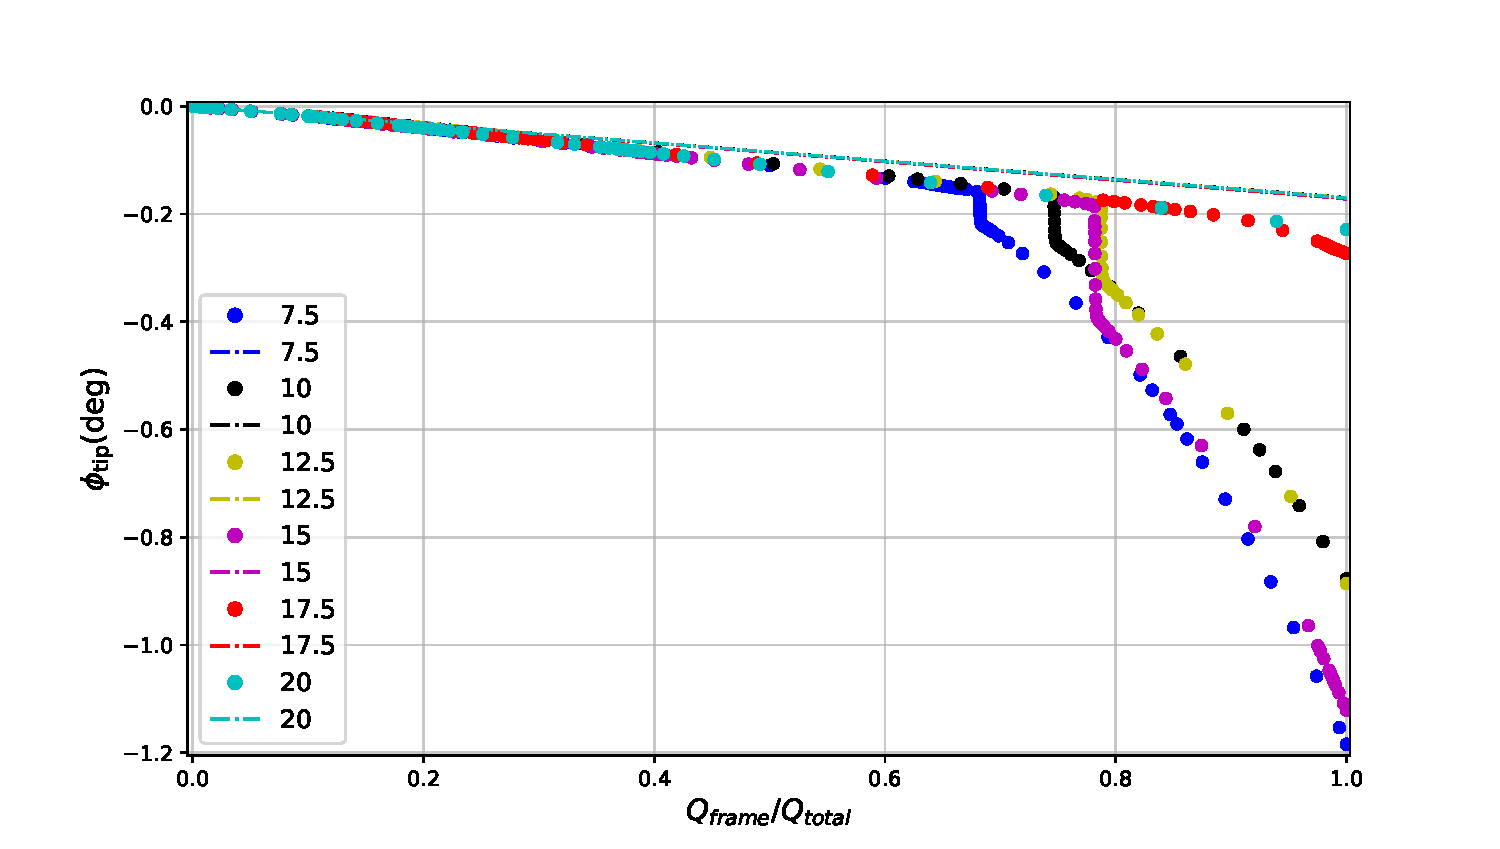
\includegraphics[width=0.8 \textwidth]{../figures/result-sim/r/force_displacement-far}
        \caption[Force-displacement curve for various values of the chiral ligament half length]{Force-displacement curve for various values of the chiral ligament half length \chiL. The bigger the ligament half length is, the earlier that the structure will collapse after severe buckling of the ligaments at the root.}\label{fig:forceDisplacement-far-L}
      \end{figure}

    \clearpage
    \subsubsection{Chiral structure thickness $t_{\mathrm{chiral}}$}
      %

      The results for the parametric study performed on the chiral structure thickness \chit are shown in Table \ref{tab:para_chi_t}. The force-displacement curve is shown in Figure \ref{fig:forceDisplacement-far-chiral-t}. Here it can be seen that a thicker chiral structure delays the structure collapse. Similarly as it occurred for the chiral node depth \chiB, the more bigger the thickness \chit is, the more abrupt is the decrement in tip twist is. 

      \begin{table}[!htpb] %Results of chiral thickness 
        \centering
        \begin{tabular}{|l|l|l|l|l|l|l|l|l|}
        \hline
        \chit & $\phi_{\mathrm{tip}}$ (deg) & $e(\phi_{\mathrm{tip}}) (\%)$ & $\tilde{\phi}_{\mathrm{tip}}$ (deg) & $e(\tilde{\phi}_{\mathrm{tip}}) (\%)$ & $v_{\mathrm{max}}$ & $\hat{z}_{v_{\mathrm{max}}}$ & $\hat{x}_{v_{\mathrm{max}}}$ \\ \hline
        0.2 & -1.201 & 9.464 & -0.199 & -10.637 & -11.878 & 1 & 0.334 \\ \hline
        0.4 & -1.026 & 9.503 & -0.179 & -10.334 & -10.896 & 1 & 0.334 \\ \hline
        0.6 & -0.922 & 13.874 & -0.164 & -9.816 & -10.036 & 1 & 0.334 \\ \hline
        0.8 & -0.232 & 14.445 & -0.15 & -9.323 & -1.449 & 1 & 0.971 \\ \hline
        \end{tabular}
        \caption[Results from parametric study on chiral structure thickness]{Results from parametric study on chiral structure thickness \chit. The results show the twist at the tip of the wing-box for the Abaqus nonlinear simulation $\phi_{\mathrm{tip}}$ and for the linear simulation $\tilde{\phi}_{\mathrm{tip}}$. The maximum relative error of the mean calculation, expressed as percentage, for these two magnitudes is $e(\phi_{\mathrm{tip}})$ and $e(\tilde{\phi}_{\mathrm{tip}})$, respectively. The table also shows the maximum vertical displacement $v_{\mathrm{max}}$ among all the mesh nodes located on the upper skin of the wing-box and the dimensionless position in the spanwise direction $\hat{x}_{v_{\mathrm{max}}}$ and in the chordwise direction $\hat{z}_{v_{\mathrm{max}}}$ of the node that shows $v = v_{\mathrm{max}}$.}
        \label{tab:para_chi_t}
      \end{table}

      \begin{figure}[!htpb] %force_displacement-far
        \centering
        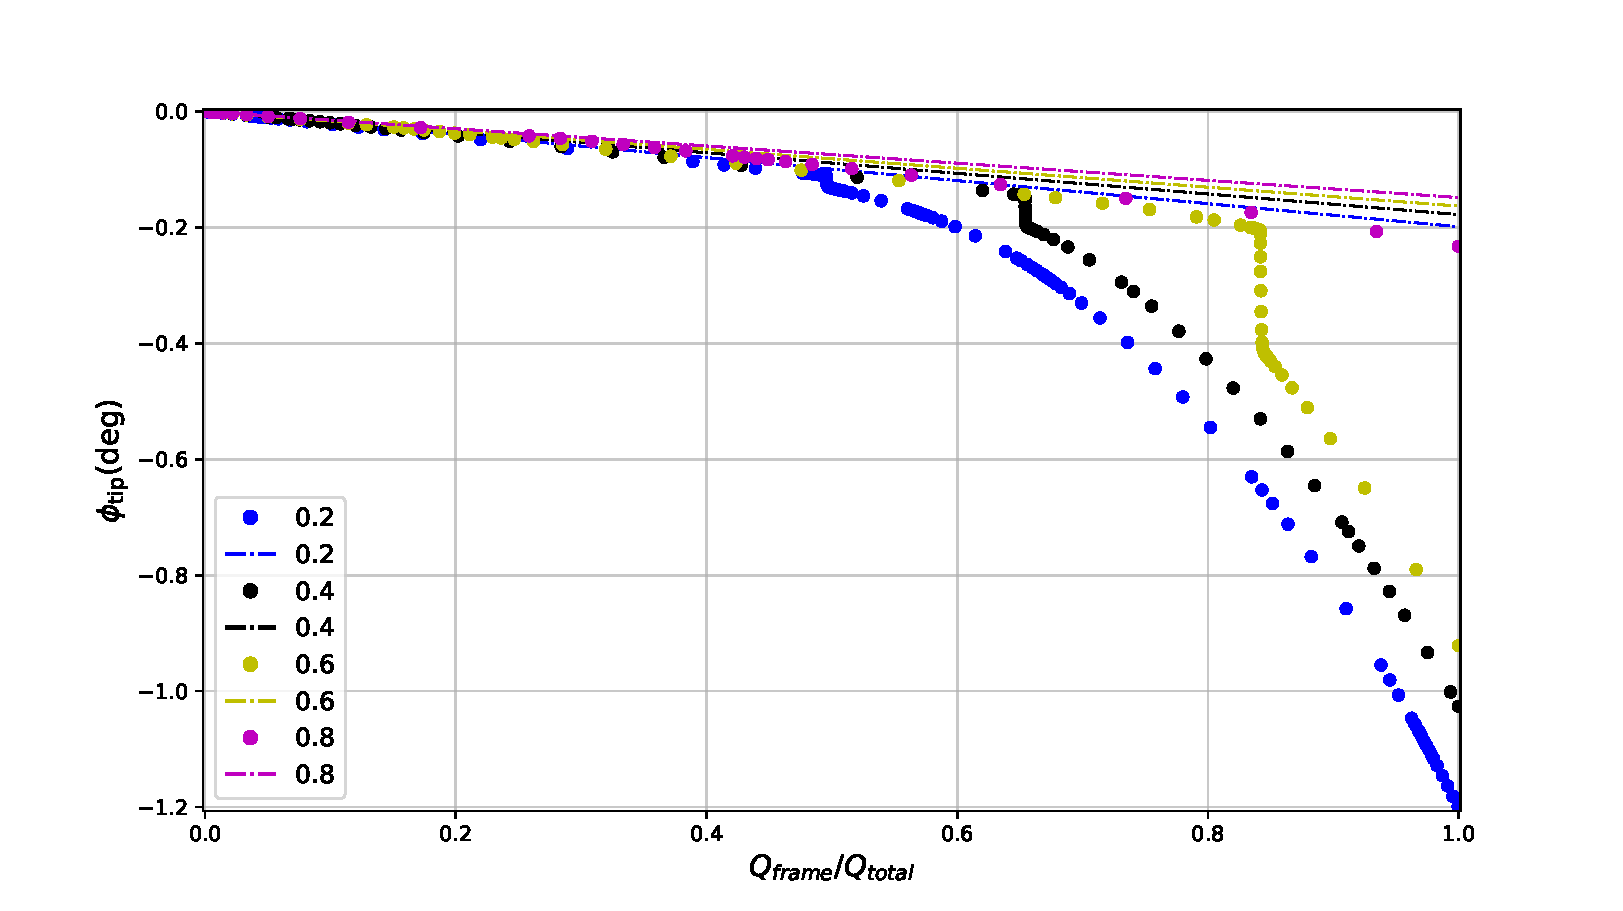
\includegraphics[width=0. \textwidth]{../figures/result-sim/chiral_t/force_displacement-far}
        \caption[Force-displacement curve for various values of the chiral structure thickness]{Force-displacement curve for various values of the chiral structure thickness \chit. The bigger the ligament half length is, the earlier that the structure will collapse after severe buckling of the ligaments at the root.}\label{fig:forceDisplacement-far-chiral-t}
      \end{figure}